\KOMAoption{paper}{a4, portrait}
\areaset{267mm}{180mm}
\fancyheadoffset{0pt} % обновляем хедер и футер

\newgeometry{
  top=14mm,
  bottom=11mm,
  right=10mm,
  left=22mm,
}

\begin{landscape}

%\setlength{\headsep}{5.6mm} 
%\setlength{\topmargin}{-27mm}
\setlength{\footskip}{15.5pt}
%\setlength{\textwidth}{305mm}

\color{uniblue}{\section[(справочное) Перечень сигналов ФСУ, предназначенных для \newline конфигурирования устройства <<ЮНИТ-М300-Т>>]{(справочное)\\Перечень сигналов ФСУ, предназначенных для конфигурирования устройства <<ЮНИТ-М300-Т>>}\label{app:signals}}
\color{black}

\begin{enumerate}[label=\ref{app:signals}.\arabic*] % Без глобального влияния
  \item Перечень сигналов самодиагностики, доступных для конфигурирования, приведен в документации ЮТКБ.656122.609 РЭ <<Устройство защиты и автоматики серии <<ЮНИТ-М300>>. Руководство по эксплуатации общее>>.
  \item Условные обозначения, применяемые в таблице перечня сигналов:
  \begin{itemize}
    \item[$\text{(--)}$] { - сигнал не имеет возможности конфигурации на данный параметр;}
    \item[$\text{(+)}$] { - сигнал имеет возможность конфигурации на данный параметр.}
  \end{itemize}
\end{enumerate}

\small % сделаем шрифт в таблице поменьше
% В таблице ниже убрал правую и левую горизонтальные линии чтобы не сливались и жирно видно - также в настройках geometry прищлось поле right =8mm а не 5 mm 
% так как строки ниже колонтитулов спускались
\begin{longtable}{
>{\centering\arraybackslash}m{6.0cm}
|>{\centering\arraybackslash}m{3.45cm}
|>{\centering\arraybackslash}m{2cm}
|>{\centering\arraybackslash}m{2cm}
|>{\centering\arraybackslash}m{2cm}
|>{\centering\arraybackslash}m{2cm}
|>{\centering\arraybackslash}m{2cm}
|>{\centering\arraybackslash}m{2cm}
|>{\centering\arraybackslash}m{2.107cm}
}

%\caption{Перечень сигналов ФСУ, предназначенных для конфигурирования устройств ЮНИТ-М300\vspace{-0.5\baselineskip}}\label{appA:tbl1}\\ % выравнивает надпись посередине таблицы
\caption{Перечень сигналов ФСУ, предназначенных для конфигурирования устройства\hfill\vspace{-0.5\baselineskip}}\label{appA:tbl1}\\ 

\hline
\rowcolor{gray!20}
Полное наименование сигнала & Наименование сигнала на ФСУ & Дискретные входы & Выходные реле & Светодиоды & Функционал. клавиши & Регистратор событий & Аварийный осциллограф & Пуск авар. осциллографа \\ 
\hline
\endfirsthead
%\caption{\emph{Продолжение\vspace{-0.5\baselineskip}}} \\ % Отступ обозначения таблицы от таблицы и выравнивание надписи слева
\caption*{\hspace{3pt}\emph{Продолжение таблицы \ref{appA:tbl1}\hfill\vspace{-0.5\baselineskip}}} \\ % сделано по ГОСТ 2.105 п.6.8.7
\hline
\rowcolor{gray!20}
Полное наименование сигнала & Наименование сигнала на ФСУ & Дискретные входы & Выходные реле & Светодиоды & Функционал. клавиши & Регистратор событий & Аварийный осциллограф & Пуск авар. осциллографа \\ 
%\hline
\endhead

%\hline
\endfoot

%\hline
\endlastfoot

%===t2
\rowcolor{gray!10}
\multicolumn{9}{c}{Общие сигналы ФС} \\
\hline
\raggedright СВ НН включен & \centering СВ НН включен & \centering + & \centering + & \centering + & \centering -- & \centering + & \centering + & \centering \arraybackslash + \\ \hline
\raggedright В НН включен & \centering В НН включен & \centering + & \centering + & \centering + & \centering -- & \centering + & \centering + & \centering \arraybackslash + \\ \hline
\raggedright Срабатывание внешнего КПОН & \centering КПОН внеш. & \centering + & \centering + & \centering + & \centering -- & \centering + & \centering + & \centering \arraybackslash + \\ \hline
\raggedright Внешний пуск ЛЗТ & \centering Внеш. пуск ЛЗТ & \centering + & \centering + & \centering + & \centering -- & \centering + & \centering + & \centering \arraybackslash + \\ \hline
\raggedright Блокировка ЛЗТ & \centering Блокировка ЛЗТ & \centering + & \centering + & \centering + & \centering -- & \centering + & \centering + & \centering \arraybackslash + \\ \hline
\raggedright Срабатывание внешнего БНН & \centering Сраб БНН внеш & \centering + & \centering + & \centering + & \centering -- & \centering + & \centering + & \centering \arraybackslash + \\ \hline
\raggedright Срабатывание сигнального контакта газового реле & \centering Сигн.конт.газ.реле & \centering + & \centering + & \centering + & \centering -- & \centering + & \centering + & \centering \arraybackslash + \\ \hline
\raggedright Срабатывание устройства контроля изоляции ГЗсигн & \centering Сраб. КИ ГЗсигн & \centering + & \centering + & \centering + & \centering -- & \centering + & \centering + & \centering \arraybackslash + \\ \hline
\raggedright Срабатывание отключающего контакта газового реле & \centering Откл.конт.газ.реле & \centering + & \centering + & \centering + & \centering -- & \centering + & \centering + & \centering \arraybackslash + \\ \hline
\raggedright Срабатывание устройства контроля изоляции ГЗоткл & \centering Сраб. КИ ГЗоткл & \centering + & \centering + & \centering + & \centering -- & \centering + & \centering + & \centering \arraybackslash + \\ \hline
\raggedright Срабатывание контакта струйного реле РПН & \centering Конт.струйн. реле & \centering + & \centering + & \centering + & \centering -- & \centering + & \centering + & \centering \arraybackslash + \\ \hline
\raggedright Срабатывание устройства контроля изоляция ГЗ РПН & \centering Сраб. КИ ГЗ РПН & \centering + & \centering + & \centering + & \centering -- & \centering + & \centering + & \centering \arraybackslash + \\ \hline
\raggedright Повышенная температура масла & \centering Повыш. t масла & \centering + & \centering + & \centering + & \centering -- & \centering + & \centering + & \centering \arraybackslash + \\ \hline
\raggedright Аварийная температура масла & \centering Авар. t масла & \centering + & \centering + & \centering + & \centering -- & \centering + & \centering + & \centering \arraybackslash + \\ \hline
\raggedright Срабатывание устройства контроля изоляции датчика температуры масла & \centering Сраб. КИ ДТм & \centering + & \centering + & \centering + & \centering -- & \centering + & \centering + & \centering \arraybackslash + \\ \hline
\raggedright Повышенная температура обмотки & \centering Повыш. t обмотки & \centering + & \centering + & \centering + & \centering -- & \centering + & \centering + & \centering \arraybackslash + \\ \hline
\raggedright Аварийная температура обмотки & \centering Авар. t обмотки & \centering + & \centering + & \centering + & \centering -- & \centering + & \centering + & \centering \arraybackslash + \\ \hline
\raggedright Срабатывание устройства контроля изоляции датчика температуры обмотки & \centering Сраб. КИ ДТо & \centering + & \centering + & \centering + & \centering -- & \centering + & \centering + & \centering \arraybackslash + \\ \hline
\raggedright Срабатывание датчика давления & \centering Сраб.датч.давл. & \centering + & \centering + & \centering + & \centering -- & \centering + & \centering + & \centering \arraybackslash + \\ \hline
\raggedright Срабатывание устройства контроля изоляции датчика давления & \centering Сраб. КИ датч.давл. & \centering + & \centering + & \centering + & \centering -- & \centering + & \centering + & \centering \arraybackslash + \\ \hline
\raggedright Высокий уровень масла трансформатора & \centering Выс.ур.масла тр. & \centering + & \centering + & \centering + & \centering -- & \centering + & \centering + & \centering \arraybackslash + \\ \hline
\raggedright Низкий уровень масла трансформатора & \centering Низк.ур.масла тр. & \centering + & \centering + & \centering + & \centering -- & \centering + & \centering + & \centering \arraybackslash + \\ \hline
\raggedright Высокий уровень масла РПН & \centering Выс.ур.масла РПН & \centering + & \centering + & \centering + & \centering -- & \centering + & \centering + & \centering \arraybackslash + \\ \hline
\raggedright Низкий уровень масла РПН & \centering Низк.ур.масла РПН & \centering + & \centering + & \centering + & \centering -- & \centering + & \centering + & \centering \arraybackslash + \\ \hline
\raggedright Срабатывание предупредительного клапана & \centering Сраб.пред.клапана & \centering + & \centering + & \centering + & \centering -- & \centering + & \centering + & \centering \arraybackslash + \\ \hline
\raggedright Срабатывание отсечного клапана & \centering Сраб.отсеч.клапана & \centering + & \centering + & \centering + & \centering -- & \centering + & \centering + & \centering \arraybackslash + \\ \hline
\raggedright Низкая температура масла РПН & \centering Низк. t масла РПН & \centering + & \centering + & \centering + & \centering -- & \centering + & \centering + & \centering \arraybackslash + \\ \hline
\raggedright Внешнее отключение от ЗДЗ НН & \centering Внеш.откл. от ЗДЗ & \centering + & \centering + & \centering + & \centering -- & \centering + & \centering + & \centering \arraybackslash + \\ \hline
\raggedright Внешнее отключение от УРОВ НН & \centering Внеш.откл. от УРОВ & \centering + & \centering + & \centering + & \centering -- & \centering + & \centering + & \centering \arraybackslash + \\ \hline
\raggedright Контроль цепи ЭМВ & \centering Контроль цепи ЭМВ & \centering + & \centering + & \centering + & \centering -- & \centering + & \centering + & \centering \arraybackslash + \\ \hline
\raggedright Контроль цепи ЭМО1 & \centering Контроль цепи ЭМО1 & \centering + & \centering + & \centering + & \centering -- & \centering + & \centering + & \centering \arraybackslash + \\ \hline
\raggedright Контроль цепи ЭМО2 & \centering Контроль цепи ЭМО2 & \centering + & \centering + & \centering + & \centering -- & \centering + & \centering + & \centering \arraybackslash + \\ \hline
\raggedright Пуск УРОВ внешний & \centering Пуск УРОВ внешний & \centering + & \centering + & \centering + & \centering -- & \centering + & \centering + & \centering \arraybackslash + \\ \hline
\raggedright Контроль оперативного тока ЭМО1, ЭМВ & \centering ОТ цепей ЭМО1,ЭМВ & \centering + & \centering + & \centering + & \centering -- & \centering + & \centering + & \centering \arraybackslash + \\ \hline
\raggedright Контроль оперативного тока ЭМО2 & \centering ОТ цепей ЭМО2 & \centering + & \centering + & \centering + & \centering -- & \centering + & \centering + & \centering \arraybackslash + \\ \hline
\raggedright Аварийный уровень изоляции В & \centering Авар.уров.изоляц. В & \centering + & \centering + & \centering + & \centering -- & \centering + & \centering + & \centering \arraybackslash + \\ \hline
\raggedright Низкий уровень изоляции В & \centering Низ.уров.изоляц. В & \centering + & \centering + & \centering + & \centering -- & \centering + & \centering + & \centering \arraybackslash + \\ \hline
\raggedright Пружина не заведена & \centering Пружина не заведена & \centering + & \centering + & \centering + & \centering -- & \centering + & \centering + & \centering \arraybackslash + \\ \hline
\raggedright Работа ЭМВ & \centering Работа ЭМВ & \centering + & \centering + & \centering + & \centering -- & \centering + & \centering + & \centering \arraybackslash + \\ \hline
\raggedright Работа ЭМО1 & \centering Работа ЭМО1 & \centering + & \centering + & \centering + & \centering -- & \centering + & \centering + & \centering \arraybackslash + \\ \hline
\raggedright Работа ЭМО2 & \centering Работа ЭМО2 & \centering + & \centering + & \centering + & \centering -- & \centering + & \centering + & \centering \arraybackslash + \\ \hline
\raggedright Отключение от кнопки & \centering Откл. от кнопки & \centering + & \centering + & \centering + & \centering -- & \centering + & \centering + & \centering \arraybackslash + \\ \hline
\raggedright Внешняя блокировка управления В & \centering Внеш. блок. упр. В & \centering + & \centering + & \centering + & \centering -- & \centering + & \centering + & \centering \arraybackslash + \\ \hline
\raggedright Ключ М/Д привода В & \centering Ключ М/Д привода В & \centering + & \centering + & \centering + & \centering -- & \centering + & \centering + & \centering \arraybackslash + \\ \hline
\raggedright Отключить В от пульта управления & \centering Отключить В от ПУ & \centering + & \centering + & \centering + & \centering -- & \centering + & \centering + & \centering \arraybackslash + \\ \hline
\raggedright Отключить В от телеуправления & \centering Отключить В от ТУ & \centering + & \centering + & \centering + & \centering -- & \centering + & \centering + & \centering \arraybackslash + \\ \hline
\raggedright Включить В от пульта управления & \centering Включить В от ПУ & \centering + & \centering + & \centering + & \centering -- & \centering + & \centering + & \centering \arraybackslash + \\ \hline
\raggedright Включить В от телеуправления & \centering Включить В от ТУ & \centering + & \centering + & \centering + & \centering -- & \centering + & \centering + & \centering \arraybackslash + \\ \hline
\raggedright Выключатель отключен (блок контакт) & \centering В отключен (б/к) & \centering + & \centering + & \centering + & \centering -- & \centering + & \centering + & \centering \arraybackslash + \\ \hline
\raggedright Выключатель включен (блок контакт) & \centering В включен (б/к) & \centering + & \centering + & \centering + & \centering -- & \centering + & \centering + & \centering \arraybackslash + \\ \hline
\raggedright Контроль оперативного тока цепей ГЗ & \centering ОТ цепей ГЗ & \centering + & \centering + & \centering + & \centering -- & \centering + & \centering + & \centering \arraybackslash + \\ \hline
\raggedright Контроль оперативного тока цепей ТЗ, ТС & \centering ОТ цепей ТЗ, ТС & \centering + & \centering + & \centering + & \centering -- & \centering + & \centering + & \centering \arraybackslash + \\ \hline
\raggedright Контроль оперативного тока цепей ЗДЗ НН & \centering ОТ цепей ЗДЗ НН & \centering + & \centering + & \centering + & \centering -- & \centering + & \centering + & \centering \arraybackslash + \\ \hline
\raggedright Контроль оперативного тока цепей УРОВ НН & \centering ОТ цепей УРОВ НН & \centering + & \centering + & \centering + & \centering -- & \centering + & \centering + & \centering \arraybackslash + \\ \hline
\raggedright Контроль оперативного тока ИЭУ ТН & \centering ОТ ИЭУ ТН & \centering + & \centering + & \centering + & \centering -- & \centering + & \centering + & \centering \arraybackslash + \\ \hline
\raggedright Неисправность опер. тока цепей сигнализации выключателя & \centering ОТ цепей сигн. В & \centering + & \centering + & \centering + & \centering -- & \centering + & \centering + & \centering \arraybackslash + \\ \hline
\raggedright Положение двери шкафа & \centering Дверь шкафа & \centering + & \centering + & \centering + & \centering -- & \centering + & \centering + & \centering \arraybackslash + \\ \hline
\raggedright Положение переключателя SA1 цепей управления & \centering Положение SA1 & \centering + & \centering + & \centering + & \centering -- & \centering + & \centering + & \centering \arraybackslash + \\ \hline
\raggedright Положение переключателя SA2 цепей управления & \centering Положение SA2 & \centering + & \centering + & \centering + & \centering -- & \centering + & \centering + & \centering \arraybackslash + \\ \hline
\raggedright Положение переключателя SA3 цепей управления & \centering Положение SA3 & \centering + & \centering + & \centering + & \centering -- & \centering + & \centering + & \centering \arraybackslash + \\ \hline
\raggedright Положение переключателя SA4 цепей управления & \centering Положение SA4 & \centering + & \centering + & \centering + & \centering -- & \centering + & \centering + & \centering \arraybackslash + \\ \hline
\raggedright Положение переключателя SA5 цепей управления & \centering Положение SA5 & \centering + & \centering + & \centering + & \centering -- & \centering + & \centering + & \centering \arraybackslash + \\ \hline
\raggedright Положение испытательного блока SG1 & \centering Положение SG1 & \centering + & \centering + & \centering + & \centering -- & \centering + & \centering + & \centering \arraybackslash + \\ \hline
\raggedright Положение испытательного блока SG2 & \centering Положение SG2 & \centering + & \centering + & \centering + & \centering -- & \centering + & \centering + & \centering \arraybackslash + \\ \hline
\raggedright Сигнал внешний 1 & \centering Сигнал внешний 1 & \centering + & \centering + & \centering + & \centering -- & \centering + & \centering + & \centering \arraybackslash + \\ \hline
\raggedright Сигнал внешний 2 & \centering Сигнал внешний 2 & \centering + & \centering + & \centering + & \centering -- & \centering + & \centering + & \centering \arraybackslash + \\ \hline
\raggedright Сигнал внешний 3 & \centering Сигнал внешний 3 & \centering + & \centering + & \centering + & \centering -- & \centering + & \centering + & \centering \arraybackslash + \\ \hline
\raggedright Сигнал внешний 4 & \centering Сигнал внешний 4 & \centering + & \centering + & \centering + & \centering -- & \centering + & \centering + & \centering \arraybackslash + \\ \hline
\raggedright Оперативно отключить В & \centering Опер. отключить В & \centering + & \centering + & \centering + & \centering -- & \centering + & \centering + & \centering \arraybackslash + \\ \hline
\raggedright Оперативно включить В & \centering Опер. включить В & \centering + & \centering + & \centering + & \centering -- & \centering + & \centering + & \centering \arraybackslash + \\ \hline
\raggedright Отключить В с ИЧМ & \centering Откл. В ИЧМ & \centering + & \centering + & \centering + & \centering -- & \centering + & \centering + & \centering \arraybackslash + \\ \hline
\raggedright Включить В с ИЧМ & \centering Вкл. В ИЧМ & \centering + & \centering + & \centering + & \centering -- & \centering + & \centering + & \centering \arraybackslash + \\ \hline
\raggedright Сброс & \centering Сброс & \centering + & \centering + & \centering + & \centering -- & \centering + & \centering + & \centering \arraybackslash + \\ \hline
\raggedright Сброс счетчика операций В & \centering Сброс счет.опер.В & \centering + & \centering + & \centering + & \centering -- & \centering + & \centering + & \centering \arraybackslash + \\ \hline
\raggedright Внутренняя неисправность & \centering IRF & \centering + & \centering + & \centering + & \centering -- & \centering + & \centering + & \centering \arraybackslash + \\ \hline
\raggedright Test/blocked & \centering Test/blocked & \centering + & \centering + & \centering + & \centering -- & \centering + & \centering + & \centering \arraybackslash + \\ \hline
\raggedright Поведение местного управления & \centering Повед. местн. упр. & \centering + & \centering + & \centering + & \centering -- & \centering + & \centering + & \centering \arraybackslash + \\ \hline
\raggedright Положение ключа режима управления & \centering Ключ упр. & \centering + & \centering + & \centering + & \centering -- & \centering + & \centering + & \centering \arraybackslash + \\ \hline
\raggedright Право на переключение на уровне станции & \centering Перекл. ур. станц. & \centering + & \centering + & \centering + & \centering -- & \centering + & \centering + & \centering \arraybackslash + \\ \hline
\raggedright Критическая неисправность & \centering Неисправность & \centering + & \centering -- & \centering + & \centering -- & \centering + & \centering + & \centering \arraybackslash + \\ \hline
\raggedright Некритическая ошибка & \centering Ошибка & \centering + & \centering -- & \centering + & \centering -- & \centering + & \centering + & \centering \arraybackslash + \\ \hline
\raggedright Оперативный вывод терминала от ФК & \centering ФК: Вывод терминала & \centering -- & \centering -- & \centering -- & \centering + & \centering + & \centering + & \centering \arraybackslash + \\ \hline
\raggedright Оперативный вывод терминала от ДВ & \centering ДВ: Вывод терминала & \centering + & \centering -- & \centering -- & \centering -- & \centering + & \centering + & \centering \arraybackslash + \\ \hline
\raggedright Оперативный вывод МТЗ от ФК & \centering ФК: ОВ МТЗ & \centering -- & \centering -- & \centering -- & \centering + & \centering + & \centering + & \centering \arraybackslash + \\ \hline
\raggedright Оперативный вывод МТЗ от ДВ & \centering ДВ: ОВ МТЗ & \centering + & \centering -- & \centering -- & \centering -- & \centering + & \centering + & \centering \arraybackslash + \\ \hline
\raggedright Оперативный вывод 1 ступени МТЗ от ФК & \centering ФК: ОВ МТЗ 1 ст & \centering -- & \centering -- & \centering -- & \centering + & \centering + & \centering + & \centering \arraybackslash + \\ \hline
\raggedright Оперативный вывод 1 ступени МТЗ от ДВ & \centering ДВ: ОВ МТЗ 1 ст & \centering + & \centering -- & \centering -- & \centering -- & \centering + & \centering + & \centering \arraybackslash + \\ \hline
\raggedright Оперативный вывод 2 ступени МТЗ от ФК & \centering ФК: ОВ МТЗ 2 ст & \centering -- & \centering -- & \centering -- & \centering + & \centering + & \centering + & \centering \arraybackslash + \\ \hline
\raggedright Оперативный вывод 2 ступени МТЗ от ДВ & \centering ДВ: ОВ МТЗ 2 ст & \centering + & \centering -- & \centering -- & \centering -- & \centering + & \centering + & \centering \arraybackslash + \\ \hline
\raggedright Оперативный вывод 3 ступени МТЗ от ФК & \centering ФК: ОВ МТЗ 3 ст & \centering -- & \centering -- & \centering -- & \centering + & \centering + & \centering + & \centering \arraybackslash + \\ \hline
\raggedright Оперативный вывод 3 ступени МТЗ от ДВ & \centering ДВ: ОВ МТЗ 3 ст & \centering + & \centering -- & \centering -- & \centering -- & \centering + & \centering + & \centering \arraybackslash + \\ \hline
\raggedright Перевод МТЗ 1 ступени на сигнал от ФК & \centering ФК: МТЗ 1 ст на сигн & \centering -- & \centering -- & \centering -- & \centering + & \centering + & \centering + & \centering \arraybackslash + \\ \hline
\raggedright Перевод МТЗ 1 ступени на сигнал от ДВ & \centering ДВ: МТЗ 1 ст на сигн & \centering + & \centering -- & \centering -- & \centering -- & \centering + & \centering + & \centering \arraybackslash + \\ \hline
\raggedright Перевод МТЗ 2 ступени на сигнал от ФК & \centering ФК: МТЗ 2 ст на сигн & \centering -- & \centering -- & \centering -- & \centering + & \centering + & \centering + & \centering \arraybackslash + \\ \hline
\raggedright Перевод МТЗ 2 ступени на сигнал от ДВ & \centering ДВ: МТЗ 2 ст на сигн & \centering + & \centering -- & \centering -- & \centering -- & \centering + & \centering + & \centering \arraybackslash + \\ \hline
\raggedright Перевод МТЗ 3 ступени на сигнал от ФК & \centering ФК: МТЗ 3 ст на сигн & \centering -- & \centering -- & \centering -- & \centering + & \centering + & \centering + & \centering \arraybackslash + \\ \hline
\raggedright Перевод МТЗ 3 ступени на сигнал от ДВ & \centering ДВ: МТЗ 3 ст на сигн & \centering + & \centering -- & \centering -- & \centering -- & \centering + & \centering + & \centering \arraybackslash + \\ \hline
\raggedright Оперативный вывод ТО от ФК & \centering ФК: ОВ ТО & \centering -- & \centering -- & \centering -- & \centering + & \centering + & \centering + & \centering \arraybackslash + \\ \hline
\raggedright Оперативный вывод ТО от ДВ & \centering ДВ: ОВ ТО & \centering + & \centering -- & \centering -- & \centering -- & \centering + & \centering + & \centering \arraybackslash + \\ \hline
\raggedright Перевод ТО на сигнал от ФК & \centering ФК: ТО на сигн & \centering -- & \centering -- & \centering -- & \centering + & \centering + & \centering + & \centering \arraybackslash + \\ \hline
\raggedright Перевод ТО на сигнал от ДВ & \centering ДВ: ТО на сигн & \centering + & \centering -- & \centering -- & \centering -- & \centering + & \centering + & \centering \arraybackslash + \\ \hline
\raggedright Оперативный вывод ЛЗТ от ФК & \centering ФК: ОВ ЛЗТ & \centering -- & \centering -- & \centering -- & \centering + & \centering + & \centering + & \centering \arraybackslash + \\ \hline
\raggedright Оперативный вывод ЛЗТ от ДВ & \centering ДВ: ОВ ЛЗТ & \centering + & \centering -- & \centering -- & \centering -- & \centering + & \centering + & \centering \arraybackslash + \\ \hline
\raggedright Оперативный вывод ЗП от ФК & \centering ФК: ОВ ЗП & \centering -- & \centering -- & \centering -- & \centering + & \centering + & \centering + & \centering \arraybackslash + \\ \hline
\raggedright Оперативный вывод ЗП от ДВ & \centering ДВ: ОВ ЗП & \centering + & \centering -- & \centering -- & \centering -- & \centering + & \centering + & \centering \arraybackslash + \\ \hline
\raggedright Перевод ЗП на отключение от ФК & \centering ФК: ЗП на откл & \centering -- & \centering -- & \centering -- & \centering + & \centering + & \centering + & \centering \arraybackslash + \\ \hline
\raggedright Перевод ЗП на отключение от ДВ & \centering ДВ: ЗП на откл & \centering + & \centering -- & \centering -- & \centering -- & \centering + & \centering + & \centering \arraybackslash + \\ \hline
\raggedright Оперативный вывод ЗОП от ФК & \centering ФК: ОВ ЗОП & \centering -- & \centering -- & \centering -- & \centering + & \centering + & \centering + & \centering \arraybackslash + \\ \hline
\raggedright Оперативный вывод ЗОП от ДВ & \centering ДВ: ОВ ЗОП & \centering + & \centering -- & \centering -- & \centering -- & \centering + & \centering + & \centering \arraybackslash + \\ \hline
\raggedright Перевод ЗОП на сигнал от ФК & \centering ФК: ЗОП на сигн & \centering -- & \centering -- & \centering -- & \centering + & \centering + & \centering + & \centering \arraybackslash + \\ \hline
\raggedright Перевод ЗОП на сигнал от ДВ & \centering ДВ: ЗОП на сигн & \centering + & \centering -- & \centering -- & \centering -- & \centering + & \centering + & \centering \arraybackslash + \\ \hline
\raggedright Оперативный вывод ТК ЗДЗ от ФК & \centering ФК: ОВ ТК ЗДЗ & \centering -- & \centering -- & \centering -- & \centering + & \centering + & \centering + & \centering \arraybackslash + \\ \hline
\raggedright Оперативный вывод ТК ЗДЗ от ДВ & \centering ДВ: ОВ ТК ЗДЗ & \centering + & \centering -- & \centering -- & \centering -- & \centering + & \centering + & \centering \arraybackslash + \\ \hline
\raggedright Оперативный вывод ТО РПН от ФК & \centering ФК: ОВ ТО РПН & \centering -- & \centering -- & \centering -- & \centering + & \centering + & \centering + & \centering \arraybackslash + \\ \hline
\raggedright Оперативный вывод ТО РПН от ДВ & \centering ДВ: ОВ ТО РПН & \centering + & \centering -- & \centering -- & \centering -- & \centering + & \centering + & \centering \arraybackslash + \\ \hline
\raggedright Оперативный вывод КЦН НН от ФК & \centering ФК: ОВ КЦН НН & \centering -- & \centering -- & \centering -- & \centering + & \centering + & \centering + & \centering \arraybackslash + \\ \hline
\raggedright Оперативный вывод КЦН НН от ДВ & \centering ДВ: ОВ КЦН НН & \centering + & \centering -- & \centering -- & \centering -- & \centering + & \centering + & \centering \arraybackslash + \\ \hline
\raggedright Оперативный вывод ЛО ГЗсигн от ФК & \centering ФК: ОВ ЛО ГЗсигн & \centering -- & \centering -- & \centering -- & \centering + & \centering + & \centering + & \centering \arraybackslash + \\ \hline
\raggedright Оперативный вывод ЛО ГЗсигн от ДВ & \centering ДВ: ОВ ЛО ГЗсигн & \centering + & \centering -- & \centering -- & \centering -- & \centering + & \centering + & \centering \arraybackslash + \\ \hline
\raggedright Перевод ЛО ГЗсигн на отключение от ФК & \centering ФК: ЛО ГЗсигн на откл & \centering -- & \centering -- & \centering -- & \centering + & \centering + & \centering + & \centering \arraybackslash + \\ \hline
\raggedright Перевод ЛО ГЗсигн на отключение от ДВ & \centering ДВ: ЛО ГЗсигн на откл & \centering + & \centering -- & \centering -- & \centering -- & \centering + & \centering + & \centering \arraybackslash + \\ \hline
\raggedright Оперативный вывод ЛО ГЗоткл от ФК & \centering ФК: ОВ ЛО ГЗоткл & \centering -- & \centering -- & \centering -- & \centering + & \centering + & \centering + & \centering \arraybackslash + \\ \hline
\raggedright Оперативный вывод ЛО ГЗоткл от ДВ & \centering ДВ: ОВ ЛО ГЗоткл & \centering + & \centering -- & \centering -- & \centering -- & \centering + & \centering + & \centering \arraybackslash + \\ \hline
\raggedright Перевод ЛО ГЗоткл на сигнал от ФК & \centering ФК: ЛО ГЗоткл на сигн & \centering -- & \centering -- & \centering -- & \centering + & \centering + & \centering + & \centering \arraybackslash + \\ \hline
\raggedright Перевод ЛО ГЗоткл на сигнал от ДВ & \centering ДВ: ЛО ГЗоткл на сигн & \centering + & \centering -- & \centering -- & \centering -- & \centering + & \centering + & \centering \arraybackslash + \\ \hline
\raggedright Оперативный вывод ЛО ГЗ РПН от ФК & \centering ФК: ОВ ЛО ГЗ РПН & \centering -- & \centering -- & \centering -- & \centering + & \centering + & \centering + & \centering \arraybackslash + \\ \hline
\raggedright Оперативный вывод ЛО ГЗ РПН от ДВ & \centering ДВ: ОВ ЛО ГЗ РПН & \centering + & \centering -- & \centering -- & \centering -- & \centering + & \centering + & \centering \arraybackslash + \\ \hline
\raggedright Перевод ЛО ГЗ РПН на сигнал от ФК & \centering ФК: ЛО ГЗ РПН на сигн & \centering -- & \centering -- & \centering -- & \centering + & \centering + & \centering + & \centering \arraybackslash + \\ \hline
\raggedright Перевод ЛО ГЗ РПН на сигнал от ДВ & \centering ДВ: ЛО ГЗ РПН на сигн & \centering + & \centering -- & \centering -- & \centering -- & \centering + & \centering + & \centering \arraybackslash + \\ \hline
\raggedright Оперативный вывод ЛО ТЗ от ФК & \centering ФК: ОВ ЛО ТЗ & \centering -- & \centering -- & \centering -- & \centering + & \centering + & \centering + & \centering \arraybackslash + \\ \hline
\raggedright Оперативный вывод ЛО ТЗ от ДВ & \centering ДВ: ОВ ЛО ТЗ & \centering + & \centering -- & \centering -- & \centering -- & \centering + & \centering + & \centering \arraybackslash + \\ \hline
\raggedright Оперативный вывод ЛО ДТм от ФК & \centering ФК: ОВ ЛО ДТм & \centering -- & \centering -- & \centering -- & \centering + & \centering + & \centering + & \centering \arraybackslash + \\ \hline
\raggedright Оперативный вывод ЛО ДТм от ДВ & \centering ДВ: ОВ ЛО ДТм & \centering + & \centering -- & \centering -- & \centering -- & \centering + & \centering + & \centering \arraybackslash + \\ \hline
\raggedright Перевод ЛО ДТм на сигнал от ФК & \centering ФК: ЛО ДТм на сигн & \centering -- & \centering -- & \centering -- & \centering + & \centering + & \centering + & \centering \arraybackslash + \\ \hline
\raggedright Перевод ЛО ДТм на сигнал от ДВ & \centering ДВ: ЛО ДТм на сигн & \centering + & \centering -- & \centering -- & \centering -- & \centering + & \centering + & \centering \arraybackslash + \\ \hline
\raggedright Оперативный вывод ЛО ДТо от ФК & \centering ФК: ОВ ЛО ДТо & \centering -- & \centering -- & \centering -- & \centering + & \centering + & \centering + & \centering \arraybackslash + \\ \hline
\raggedright Оперативный вывод ЛО ДТо от ДВ & \centering ДВ: ОВ ЛО ДТо & \centering + & \centering -- & \centering -- & \centering -- & \centering + & \centering + & \centering \arraybackslash + \\ \hline
\raggedright Перевод ЛО ДТо на сигнал от ФК & \centering ФК: ЛО ДТо на сигн & \centering -- & \centering -- & \centering -- & \centering + & \centering + & \centering + & \centering \arraybackslash + \\ \hline
\raggedright Перевод ЛО ДТо на сигнал от ДВ & \centering ДВ: ЛО ДТо на сигн & \centering + & \centering -- & \centering -- & \centering -- & \centering + & \centering + & \centering \arraybackslash + \\ \hline
\raggedright Оперативный вывод ЛО РД от ФК & \centering ФК: ОВ ЛО РД & \centering -- & \centering -- & \centering -- & \centering + & \centering + & \centering + & \centering \arraybackslash + \\ \hline
\raggedright Оперативный вывод ЛО РД от ДВ & \centering ДВ: ОВ ЛО РД & \centering + & \centering -- & \centering -- & \centering -- & \centering + & \centering + & \centering \arraybackslash + \\ \hline
\raggedright Перевод ЛО РД на сигнал от ФК & \centering ФК: ЛО РД на сигн & \centering -- & \centering -- & \centering -- & \centering + & \centering + & \centering + & \centering \arraybackslash + \\ \hline
\raggedright Перевод ЛО РД на сигнал от ДВ & \centering ДВ: ЛО РД на сигн & \centering + & \centering -- & \centering -- & \centering -- & \centering + & \centering + & \centering \arraybackslash + \\ \hline
\raggedright Оперативный вывод ЛО ТС от ФК & \centering ФК: ОВ ЛО ТС & \centering -- & \centering -- & \centering -- & \centering + & \centering + & \centering + & \centering \arraybackslash + \\ \hline
\raggedright Оперативный вывод ЛО ТС от ДВ & \centering ДВ: ОВ ЛО ТС & \centering + & \centering -- & \centering -- & \centering -- & \centering + & \centering + & \centering \arraybackslash + \\ \hline
\raggedright Оперативный вывод ЛО ПК от ФК & \centering ФК: ОВ ЛО ПК & \centering -- & \centering -- & \centering -- & \centering + & \centering + & \centering + & \centering \arraybackslash + \\ \hline
\raggedright Оперативный вывод ЛО ПК от ДВ & \centering ДВ: ОВ ЛО ПК & \centering + & \centering -- & \centering -- & \centering -- & \centering + & \centering + & \centering \arraybackslash + \\ \hline
\raggedright Перевод ЛО ПК на сигнал от ФК & \centering ФК: ЛО ПК на сигн & \centering -- & \centering -- & \centering -- & \centering + & \centering + & \centering + & \centering \arraybackslash + \\ \hline
\raggedright Перевод ЛО ПК на сигнал от ДВ & \centering ДВ: ЛО ПК на сигн & \centering + & \centering -- & \centering -- & \centering -- & \centering + & \centering + & \centering \arraybackslash + \\ \hline
\raggedright Оперативный вывод ЛО ОК от ФК & \centering ФК: ОВ ЛО ОК & \centering -- & \centering -- & \centering -- & \centering + & \centering + & \centering + & \centering \arraybackslash + \\ \hline
\raggedright Оперативный вывод ЛО ОК от ДВ & \centering ДВ: ОВ ЛО ОК & \centering + & \centering -- & \centering -- & \centering -- & \centering + & \centering + & \centering \arraybackslash + \\ \hline
\raggedright Перевод ЛО ОК на сигнал от ФК & \centering ФК: ЛО ОК на сигн & \centering -- & \centering -- & \centering -- & \centering + & \centering + & \centering + & \centering \arraybackslash + \\ \hline
\raggedright Перевод ЛО ОК на сигнал от ДВ & \centering ДВ: ЛО ОК на сигн & \centering + & \centering -- & \centering -- & \centering -- & \centering + & \centering + & \centering \arraybackslash + \\ \hline
\raggedright Оперативный вывод ЛО ДУм расширителя от ФК & \centering ФК: ОВ ЛО ДУм расшир & \centering -- & \centering -- & \centering -- & \centering + & \centering + & \centering + & \centering \arraybackslash + \\ \hline
\raggedright Оперативный вывод ЛО ДУм расширителя от ДВ & \centering ДВ: ОВ ЛО ДУм расшир & \centering + & \centering -- & \centering -- & \centering -- & \centering + & \centering + & \centering \arraybackslash + \\ \hline
\raggedright Перевод ЛО ДУм расширителя на сигнал от ФК & \centering ФК: ЛО ДУм расшир сигн & \centering -- & \centering -- & \centering -- & \centering + & \centering + & \centering + & \centering \arraybackslash + \\ \hline
\raggedright Перевод ЛО ДУм расширителя на сигнал от ДВ & \centering ДВ: ЛО ДУм расшир сигн & \centering + & \centering -- & \centering -- & \centering -- & \centering + & \centering + & \centering \arraybackslash + \\ \hline
\raggedright Оперативный вывод ЛО Т от ФК & \centering ФК: ОВ ЛО Т & \centering -- & \centering -- & \centering -- & \centering + & \centering + & \centering + & \centering \arraybackslash + \\ \hline
\raggedright Оперативный вывод ЛО Т от ДВ & \centering ДВ: ОВ ЛО Т & \centering + & \centering -- & \centering -- & \centering -- & \centering + & \centering + & \centering \arraybackslash + \\ \hline
\raggedright Оперативный вывод ЛО Т / ЛО от ФК & \centering ФК: ОВ ЛО Т / ЛО & \centering -- & \centering -- & \centering -- & \centering + & \centering + & \centering + & \centering \arraybackslash + \\ \hline
\raggedright Оперативный вывод ЛО Т / ЛО от ДВ & \centering ДВ: ОВ ЛО Т / ЛО & \centering + & \centering -- & \centering -- & \centering -- & \centering + & \centering + & \centering \arraybackslash + \\ \hline
\raggedright Оперативный вывод ЛО Т / ЗАПВ от ФК & \centering ФК: ОВ ЛО Т / ЗАПВ & \centering -- & \centering -- & \centering -- & \centering + & \centering + & \centering + & \centering \arraybackslash + \\ \hline
\raggedright Оперативный вывод ЛО Т / ЗАПВ от ДВ & \centering ДВ: ОВ ЛО Т / ЗАПВ & \centering + & \centering -- & \centering -- & \centering -- & \centering + & \centering + & \centering \arraybackslash + \\ \hline
\raggedright Оперативный вывод ЛО Т / ЗАВР от ФК & \centering ФК: ОВ ЛО Т / ЗАВР & \centering -- & \centering -- & \centering -- & \centering + & \centering + & \centering + & \centering \arraybackslash + \\ \hline
\raggedright Оперативный вывод ЛО Т / ЗАВР от ДВ & \centering ДВ: ОВ ЛО Т / ЗАВР & \centering + & \centering -- & \centering -- & \centering -- & \centering + & \centering + & \centering \arraybackslash + \\ \hline
\raggedright Оперативный вывод ЛО ВН от ФК & \centering ФК: ОВ ЛО ВН & \centering -- & \centering -- & \centering -- & \centering + & \centering + & \centering + & \centering \arraybackslash + \\ \hline
\raggedright Оперативный вывод ЛО ВН от ДВ & \centering ДВ: ОВ ЛО ВН & \centering + & \centering -- & \centering -- & \centering -- & \centering + & \centering + & \centering \arraybackslash + \\ \hline
\raggedright Оперативный вывод ЛО НН от ФК & \centering ФК: ОВ ЛО НН & \centering -- & \centering -- & \centering -- & \centering + & \centering + & \centering + & \centering \arraybackslash + \\ \hline
\raggedright Оперативный вывод ЛО НН от ДВ & \centering ДВ: ОВ ЛО НН & \centering + & \centering -- & \centering -- & \centering -- & \centering + & \centering + & \centering \arraybackslash + \\ \hline
\raggedright Оперативный вывод ЛО НН / ЛО от ФК & \centering ФК: ОВ ЛО НН / ЛО & \centering -- & \centering -- & \centering -- & \centering + & \centering + & \centering + & \centering \arraybackslash + \\ \hline
\raggedright Оперативный вывод ЛО НН / ЛО & \centering ДВ: ОВ ЛО НН / ЛО & \centering + & \centering -- & \centering -- & \centering -- & \centering + & \centering + & \centering \arraybackslash + \\ \hline
\raggedright Оперативный вывод ЛО НН / ЗАПВ от ФК & \centering ФК: ОВ ЛО НН / ЗАПВ & \centering -- & \centering -- & \centering -- & \centering + & \centering + & \centering + & \centering \arraybackslash + \\ \hline
\raggedright Оперативный вывод ЛО НН / ЗАПВ от ДВ & \centering ДВ: ОВ ЛО НН / ЗАПВ & \centering + & \centering -- & \centering -- & \centering -- & \centering + & \centering + & \centering \arraybackslash + \\ \hline
\raggedright Оперативный вывод ЛО НН / ЗАВР от ФК & \centering ФК: ОВ ЛО НН / ЗАВР & \centering -- & \centering -- & \centering -- & \centering + & \centering + & \centering + & \centering \arraybackslash + \\ \hline
\raggedright Оперативный вывод ЛО НН / ЗАВР от ДВ & \centering ДВ: ОВ ЛО НН / ЗАВР & \centering + & \centering -- & \centering -- & \centering -- & \centering + & \centering + & \centering \arraybackslash + \\ \hline
\raggedright Оперативный вывод УРОВ ВН от ФК & \centering ФК: ОВ УРОВ ВН & \centering -- & \centering -- & \centering -- & \centering + & \centering + & \centering + & \centering \arraybackslash + \\ \hline
\raggedright Оперативный вывод УРОВ ВН от ДВ & \centering ДВ: ОВ УРОВ ВН & \centering + & \centering -- & \centering -- & \centering -- & \centering + & \centering + & \centering \arraybackslash + \\ \hline
\raggedright Оперативный вывод КСВ от ФК & \centering ФК: ОВ КСВ & \centering -- & \centering -- & \centering -- & \centering + & \centering + & \centering + & \centering \arraybackslash + \\ \hline
\raggedright Оперативный вывод КСВ от ДВ & \centering ДВ: ОВ КСВ & \centering + & \centering -- & \centering -- & \centering -- & \centering + & \centering + & \centering \arraybackslash + \\ \hline
\raggedright Оперативный вывод УВ от ФК & \centering ФК: ОВ УВ & \centering -- & \centering -- & \centering -- & \centering + & \centering + & \centering + & \centering \arraybackslash + \\ \hline
\raggedright Оперативный вывод УВ от ДВ & \centering ДВ: ОВ УВ & \centering + & \centering -- & \centering -- & \centering -- & \centering + & \centering + & \centering \arraybackslash + \\ \hline
\raggedright Оперативный вывод КП от ФК & \centering ФК: ОВ КП & \centering -- & \centering -- & \centering -- & \centering + & \centering + & \centering + & \centering \arraybackslash + \\ \hline
\raggedright Оперативный вывод КП от ДВ & \centering ДВ: ОВ КП & \centering + & \centering -- & \centering -- & \centering -- & \centering + & \centering + & \centering \arraybackslash + \\ \hline
\raggedright Оперативный вывод КА от ФК & \centering ФК: ОВ КА & \centering -- & \centering -- & \centering -- & \centering + & \centering + & \centering + & \centering \arraybackslash + \\ \hline
\raggedright Оперативный вывод КА от ДВ & \centering ДВ: ОВ КА & \centering + & \centering -- & \centering -- & \centering -- & \centering + & \centering + & \centering \arraybackslash + \\ \hline
\raggedright Оперативный вывод ПДС от ФК & \centering ФК: ОВ ПДС & \centering -- & \centering -- & \centering -- & \centering + & \centering + & \centering + & \centering \arraybackslash + \\ \hline
\raggedright Оперативный вывод ПДС от ДВ & \centering ДВ: ОВ ПДС & \centering + & \centering -- & \centering -- & \centering -- & \centering + & \centering + & \centering \arraybackslash + \\ \hline
\raggedright Оперативный вывод ПДС НКУ от ФК & \centering ФК: ОВ ПДС НКУ & \centering -- & \centering -- & \centering -- & \centering + & \centering + & \centering + & \centering \arraybackslash + \\ \hline
\raggedright Оперативный вывод ПДС НКУ от ДВ & \centering ДВ: ОВ ПДС НКУ & \centering + & \centering -- & \centering -- & \centering -- & \centering + & \centering + & \centering \arraybackslash + \\ \hline
\raggedright Сброс счетчиков ресурса выключателя от ФК & \centering ФК: Сброс КРВ & \centering -- & \centering -- & \centering -- & \centering + & \centering + & \centering + & \centering \arraybackslash + \\ \hline
\raggedright Сброс счетчиков ресурса выключателя от ДВ & \centering ДВ: Сброс КРВ & \centering + & \centering -- & \centering -- & \centering -- & \centering + & \centering + & \centering \arraybackslash + \\ \hline
\rowcolor{gray!10}
\multicolumn{9}{c}{Логическая защита трансформатора (ЛЗТ)} \\
\hline
\rowcolor{gray!5}
\multicolumn{9}{c}{ЛЗТ} \\
\hline
\raggedright Функция введена в работу & \centering ЛЗТ / ЛЗТ: Ввод & \centering -- & \centering + & \centering + & \centering -- & \centering + & \centering + & \centering \arraybackslash + \\ \hline
\raggedright Функция оперативно выведена из работы & \centering ЛЗТ / ЛЗТ: Оперативный вывод & \centering -- & \centering + & \centering + & \centering -- & \centering + & \centering + & \centering \arraybackslash + \\ \hline
\raggedright Пуск & \centering ЛЗТ / ЛЗТ: Пуск & \centering -- & \centering + & \centering + & \centering -- & \centering + & \centering + & \centering \arraybackslash + \\ \hline
\raggedright Срабатывание & \centering ЛЗТ / ЛЗТ: Срабатывание & \centering -- & \centering + & \centering + & \centering -- & \centering + & \centering + & \centering \arraybackslash + \\ \hline
\rowcolor{gray!10}
\multicolumn{9}{c}{Токовая отсечка (ТО)} \\
\hline
\rowcolor{gray!5}
\multicolumn{9}{c}{ТО} \\
\hline
\raggedright Функция введена в работу & \centering ТО / ТО: Ввод & \centering -- & \centering + & \centering + & \centering -- & \centering + & \centering + & \centering \arraybackslash + \\ \hline
\raggedright Функция оперативно выведена из работы & \centering ТО / ТО: Оперативный вывод & \centering -- & \centering + & \centering + & \centering -- & \centering + & \centering + & \centering \arraybackslash + \\ \hline
\raggedright Пуск ИО максимального тока & \centering ТО / ТО: ИО Iмакс & \centering -- & \centering + & \centering + & \centering -- & \centering + & \centering + & \centering \arraybackslash + \\ \hline
\raggedright Пуск & \centering ТО / ТО: Пуск & \centering -- & \centering + & \centering + & \centering -- & \centering + & \centering + & \centering \arraybackslash + \\ \hline
\raggedright Срабатывание на сигнал & \centering ТО / ТО: Срабатывание сигн & \centering -- & \centering + & \centering + & \centering -- & \centering + & \centering + & \centering \arraybackslash + \\ \hline
\raggedright Срабатывание & \centering ТО / ТО: Срабатывание & \centering -- & \centering + & \centering + & \centering -- & \centering + & \centering + & \centering \arraybackslash + \\ \hline
\rowcolor{gray!10}
\multicolumn{9}{c}{Максимальная токовая защита (МТЗ)} \\
\hline
\rowcolor{gray!5}
\multicolumn{9}{c}{МТЗ 1 ст} \\
\hline
\raggedright Функция введена в работу & \centering МТЗ / МТЗ 1 ст: Ввод & \centering -- & \centering + & \centering + & \centering -- & \centering + & \centering + & \centering \arraybackslash + \\ \hline
\raggedright Функция оперативно выведена из работы & \centering МТЗ / МТЗ 1 ст: Оперативный вывод & \centering -- & \centering + & \centering + & \centering -- & \centering + & \centering + & \centering \arraybackslash + \\ \hline
\raggedright Пуск ИО тока по фазе A & \centering МТЗ / МТЗ 1 ст: ИО IA & \centering -- & \centering + & \centering + & \centering -- & \centering + & \centering + & \centering \arraybackslash + \\ \hline
\raggedright Пуск ИО тока по фазе B & \centering МТЗ / МТЗ 1 ст: ИО IB & \centering -- & \centering + & \centering + & \centering -- & \centering + & \centering + & \centering \arraybackslash + \\ \hline
\raggedright Пуск ИО тока по фазе C & \centering МТЗ / МТЗ 1 ст: ИО IC & \centering -- & \centering + & \centering + & \centering -- & \centering + & \centering + & \centering \arraybackslash + \\ \hline
\raggedright Пуск по фазе A & \centering МТЗ / МТЗ 1 ст: Пуск ф.A & \centering -- & \centering + & \centering + & \centering -- & \centering + & \centering + & \centering \arraybackslash + \\ \hline
\raggedright Пуск по фазе B & \centering МТЗ / МТЗ 1 ст: Пуск ф.B & \centering -- & \centering + & \centering + & \centering -- & \centering + & \centering + & \centering \arraybackslash + \\ \hline
\raggedright Пуск по фазе C & \centering МТЗ / МТЗ 1 ст: Пуск ф.C & \centering -- & \centering + & \centering + & \centering -- & \centering + & \centering + & \centering \arraybackslash + \\ \hline
\raggedright Пуск & \centering МТЗ / МТЗ 1 ст: Пуск & \centering -- & \centering + & \centering + & \centering -- & \centering + & \centering + & \centering \arraybackslash + \\ \hline
\raggedright Срабатывание на сигнал & \centering МТЗ / МТЗ 1 ст: Срабатывание сигн & \centering -- & \centering + & \centering + & \centering -- & \centering + & \centering + & \centering \arraybackslash + \\ \hline
\raggedright Срабатывание & \centering МТЗ / МТЗ 1 ст: Срабатывание & \centering -- & \centering + & \centering + & \centering -- & \centering + & \centering + & \centering \arraybackslash + \\ \hline
\rowcolor{gray!5}
\multicolumn{9}{c}{МТЗ 2 ст} \\
\hline
\raggedright Функция введена в работу & \centering МТЗ / МТЗ 2 ст: Ввод & \centering -- & \centering + & \centering + & \centering -- & \centering + & \centering + & \centering \arraybackslash + \\ \hline
\raggedright Функция оперативно выведена из работы & \centering МТЗ / МТЗ 2 ст: Оперативный вывод & \centering -- & \centering + & \centering + & \centering -- & \centering + & \centering + & \centering \arraybackslash + \\ \hline
\raggedright Пуск ИО тока по фазе A & \centering МТЗ / МТЗ 2 ст: ИО IA & \centering -- & \centering + & \centering + & \centering -- & \centering + & \centering + & \centering \arraybackslash + \\ \hline
\raggedright Пуск ИО тока по фазе B & \centering МТЗ / МТЗ 2 ст: ИО IB & \centering -- & \centering + & \centering + & \centering -- & \centering + & \centering + & \centering \arraybackslash + \\ \hline
\raggedright Пуск ИО тока по фазе C & \centering МТЗ / МТЗ 2 ст: ИО IC & \centering -- & \centering + & \centering + & \centering -- & \centering + & \centering + & \centering \arraybackslash + \\ \hline
\raggedright Пуск по фазе A & \centering МТЗ / МТЗ 2 ст: Пуск ф.A & \centering -- & \centering + & \centering + & \centering -- & \centering + & \centering + & \centering \arraybackslash + \\ \hline
\raggedright Пуск по фазе B & \centering МТЗ / МТЗ 2 ст: Пуск ф.B & \centering -- & \centering + & \centering + & \centering -- & \centering + & \centering + & \centering \arraybackslash + \\ \hline
\raggedright Пуск по фазе C & \centering МТЗ / МТЗ 2 ст: Пуск ф.C & \centering -- & \centering + & \centering + & \centering -- & \centering + & \centering + & \centering \arraybackslash + \\ \hline
\raggedright Пуск & \centering МТЗ / МТЗ 2 ст: Пуск & \centering -- & \centering + & \centering + & \centering -- & \centering + & \centering + & \centering \arraybackslash + \\ \hline
\raggedright Срабатывание на сигнал & \centering МТЗ / МТЗ 2 ст: Срабатывание сигн & \centering -- & \centering + & \centering + & \centering -- & \centering + & \centering + & \centering \arraybackslash + \\ \hline
\raggedright Срабатывание & \centering МТЗ / МТЗ 2 ст: Срабатывание & \centering -- & \centering + & \centering + & \centering -- & \centering + & \centering + & \centering \arraybackslash + \\ \hline
\rowcolor{gray!5}
\multicolumn{9}{c}{МТЗ 3 ст} \\
\hline
\raggedright Функция введена в работу & \centering МТЗ / МТЗ 3 ст: Ввод & \centering -- & \centering + & \centering + & \centering -- & \centering + & \centering + & \centering \arraybackslash + \\ \hline
\raggedright Функция оперативно выведена из работы & \centering МТЗ / МТЗ 3 ст: Оперативный вывод & \centering -- & \centering + & \centering + & \centering -- & \centering + & \centering + & \centering \arraybackslash + \\ \hline
\raggedright Пуск ИО тока по фазе A & \centering МТЗ / МТЗ 3 ст: ИО IA & \centering -- & \centering + & \centering + & \centering -- & \centering + & \centering + & \centering \arraybackslash + \\ \hline
\raggedright Пуск ИО тока по фазе B & \centering МТЗ / МТЗ 3 ст: ИО IB & \centering -- & \centering + & \centering + & \centering -- & \centering + & \centering + & \centering \arraybackslash + \\ \hline
\raggedright Пуск ИО тока по фазе C & \centering МТЗ / МТЗ 3 ст: ИО IC & \centering -- & \centering + & \centering + & \centering -- & \centering + & \centering + & \centering \arraybackslash + \\ \hline
\raggedright Пуск по фазе A & \centering МТЗ / МТЗ 3 ст: Пуск ф.A & \centering -- & \centering + & \centering + & \centering -- & \centering + & \centering + & \centering \arraybackslash + \\ \hline
\raggedright Пуск по фазе B & \centering МТЗ / МТЗ 3 ст: Пуск ф.B & \centering -- & \centering + & \centering + & \centering -- & \centering + & \centering + & \centering \arraybackslash + \\ \hline
\raggedright Пуск по фазе C & \centering МТЗ / МТЗ 3 ст: Пуск ф.C & \centering -- & \centering + & \centering + & \centering -- & \centering + & \centering + & \centering \arraybackslash + \\ \hline
\raggedright Пуск & \centering МТЗ / МТЗ 3 ст: Пуск & \centering -- & \centering + & \centering + & \centering -- & \centering + & \centering + & \centering \arraybackslash + \\ \hline
\raggedright Срабатывание на сигнал & \centering МТЗ / МТЗ 3 ст: Срабатывание сигн & \centering -- & \centering + & \centering + & \centering -- & \centering + & \centering + & \centering \arraybackslash + \\ \hline
\raggedright Срабатывание & \centering МТЗ / МТЗ 3 ст: Срабатывание & \centering -- & \centering + & \centering + & \centering -- & \centering + & \centering + & \centering \arraybackslash + \\ \hline
\rowcolor{gray!5}
\multicolumn{9}{c}{КПОН} \\
\hline
\raggedright Пуск КПОН & \centering МТЗ / КПОН: Пуск & \centering -- & \centering + & \centering + & \centering -- & \centering + & \centering + & \centering \arraybackslash + \\ \hline
\rowcolor{gray!5}
\multicolumn{9}{c}{БНТ} \\
\hline
\raggedright Пуск БНТ по фазе A & \centering МТЗ / БНТ: Пуск ф.A & \centering -- & \centering + & \centering + & \centering -- & \centering + & \centering + & \centering \arraybackslash + \\ \hline
\raggedright Пуск БНТ по фазе B & \centering МТЗ / БНТ: Пуск ф.B & \centering -- & \centering + & \centering + & \centering -- & \centering + & \centering + & \centering \arraybackslash + \\ \hline
\raggedright Пуск БНТ по фазе C & \centering МТЗ / БНТ: Пуск ф.C & \centering -- & \centering + & \centering + & \centering -- & \centering + & \centering + & \centering \arraybackslash + \\ \hline
\raggedright Пуск БНТ & \centering МТЗ / БНТ: Пуск & \centering -- & \centering + & \centering + & \centering -- & \centering + & \centering + & \centering \arraybackslash + \\ \hline
\rowcolor{gray!5}
\multicolumn{9}{c}{БЛЗШ} \\
\hline
\raggedright Блокировка ЛЗШ & \centering МТЗ / БЛЗШ: Блокировка & \centering -- & \centering + & \centering + & \centering -- & \centering + & \centering + & \centering \arraybackslash + \\ \hline
\rowcolor{gray!5}
\multicolumn{9}{c}{МТЗ} \\
\hline
\raggedright Пуск & \centering МТЗ / МТЗ: Пуск & \centering -- & \centering + & \centering + & \centering -- & \centering + & \centering + & \centering \arraybackslash + \\ \hline
\rowcolor{gray!10}
\multicolumn{9}{c}{Токовый контроль ЗДЗ (ТК ЗДЗ)} \\
\hline
\rowcolor{gray!5}
\multicolumn{9}{c}{ТК ЗДЗ} \\
\hline
\raggedright Функция введена в работу & \centering ТК ЗДЗ / ТК ЗДЗ: Ввод & \centering -- & \centering + & \centering + & \centering -- & \centering + & \centering + & \centering \arraybackslash + \\ \hline
\raggedright Функция оперативно выведена из работы & \centering ТК ЗДЗ / ТК ЗДЗ: Оперативный вывод & \centering -- & \centering + & \centering + & \centering -- & \centering + & \centering + & \centering \arraybackslash + \\ \hline
\raggedright Пуск ИО максимального тока & \centering ТК ЗДЗ / ТК ЗДЗ: ИО Iмакс & \centering -- & \centering + & \centering + & \centering -- & \centering + & \centering + & \centering \arraybackslash + \\ \hline
\raggedright Пуск & \centering ТК ЗДЗ / ТК ЗДЗ: Пуск & \centering -- & \centering + & \centering + & \centering -- & \centering + & \centering + & \centering \arraybackslash + \\ \hline
\rowcolor{gray!10}
\multicolumn{9}{c}{Защита от обрыва провода (ЗОП)} \\
\hline
\rowcolor{gray!5}
\multicolumn{9}{c}{ЗОП} \\
\hline
\raggedright Функция введена в работу & \centering ЗОП / ЗОП: Ввод & \centering -- & \centering + & \centering + & \centering -- & \centering + & \centering + & \centering \arraybackslash + \\ \hline
\raggedright Функция оперативно выведена из работы & \centering ЗОП / ЗОП: Оперативный вывод & \centering -- & \centering + & \centering + & \centering -- & \centering + & \centering + & \centering \arraybackslash + \\ \hline
\raggedright Пуск ИО тока обратной последовательности & \centering ЗОП / ЗОП: ИО I2 & \centering -- & \centering + & \centering + & \centering -- & \centering + & \centering + & \centering \arraybackslash + \\ \hline
\raggedright Пуск ИО по несимметрии токов прямой и обратной последовательности & \centering ЗОП / ЗОП: ИО I2/I1 & \centering -- & \centering + & \centering + & \centering -- & \centering + & \centering + & \centering \arraybackslash + \\ \hline
\raggedright Пуск & \centering ЗОП / ЗОП: Пуск & \centering -- & \centering + & \centering + & \centering -- & \centering + & \centering + & \centering \arraybackslash + \\ \hline
\raggedright Срабатывание на сигнал & \centering ЗОП / ЗОП: Срабатывание сигн & \centering -- & \centering + & \centering + & \centering -- & \centering + & \centering + & \centering \arraybackslash + \\ \hline
\raggedright Срабатывание & \centering ЗОП / ЗОП: Срабатывание & \centering -- & \centering + & \centering + & \centering -- & \centering + & \centering + & \centering \arraybackslash + \\ \hline
\rowcolor{gray!10}
\multicolumn{9}{c}{Защита от перегрузки (ЗП)} \\
\hline
\rowcolor{gray!5}
\multicolumn{9}{c}{ЗП} \\
\hline
\raggedright Функция введена в работу & \centering ЗП / ЗП: Ввод & \centering -- & \centering + & \centering + & \centering -- & \centering + & \centering + & \centering \arraybackslash + \\ \hline
\raggedright Функция оперативно выведена из работы & \centering ЗП / ЗП: Оперативный вывод & \centering -- & \centering + & \centering + & \centering -- & \centering + & \centering + & \centering \arraybackslash + \\ \hline
\raggedright Пуск ИО максимального тока & \centering ЗП / ЗП: ИО Iмакс & \centering -- & \centering + & \centering + & \centering -- & \centering + & \centering + & \centering \arraybackslash + \\ \hline
\raggedright Пуск & \centering ЗП / ЗП: Пуск & \centering -- & \centering + & \centering + & \centering -- & \centering + & \centering + & \centering \arraybackslash + \\ \hline
\raggedright Срабатывание & \centering ЗП / ЗП: Срабатывание & \centering -- & \centering + & \centering + & \centering -- & \centering + & \centering + & \centering \arraybackslash + \\ \hline
\raggedright Срабатывание на отключение & \centering ЗП / ЗП: Сраб. на откл & \centering -- & \centering + & \centering + & \centering -- & \centering + & \centering + & \centering \arraybackslash + \\ \hline
\rowcolor{gray!10}
\multicolumn{9}{c}{Токовый орган блокировки РПН (ТО РПН)} \\
\hline
\rowcolor{gray!5}
\multicolumn{9}{c}{ТО РПН} \\
\hline
\raggedright Функция введена в работу & \centering ТО РПН / ТО РПН: Ввод & \centering -- & \centering + & \centering + & \centering -- & \centering + & \centering + & \centering \arraybackslash + \\ \hline
\raggedright Функция оперативно выведена из работы & \centering ТО РПН / ТО РПН: Оперативный вывод & \centering -- & \centering + & \centering + & \centering -- & \centering + & \centering + & \centering \arraybackslash + \\ \hline
\raggedright Пуск ИО максимального тока & \centering ТО РПН / ТО РПН: ИО Iмакс & \centering -- & \centering + & \centering + & \centering -- & \centering + & \centering + & \centering \arraybackslash + \\ \hline
\raggedright Пуск & \centering ТО РПН / ТО РПН: Пуск & \centering -- & \centering + & \centering + & \centering -- & \centering + & \centering + & \centering \arraybackslash + \\ \hline
\rowcolor{gray!10}
\multicolumn{9}{c}{Логика отключения от сигнального контакта газового реле (ЛО ГЗсигн)} \\
\hline
\rowcolor{gray!5}
\multicolumn{9}{c}{ЛО} \\
\hline
\raggedright Функция введена в работу & \centering ЛО ГЗсигн / ЛО: Ввод & \centering -- & \centering + & \centering + & \centering -- & \centering + & \centering + & \centering \arraybackslash + \\ \hline
\raggedright Функция оперативно выведена из работы & \centering ЛО ГЗсигн / ЛО: Оперативный вывод & \centering -- & \centering + & \centering + & \centering -- & \centering + & \centering + & \centering \arraybackslash + \\ \hline
\raggedright Блокировка ГЗсигн & \centering ЛО ГЗсигн / ЛО: Заблокировано & \centering -- & \centering + & \centering + & \centering -- & \centering + & \centering + & \centering \arraybackslash + \\ \hline
\raggedright Срабатывание на сигнал & \centering ЛО ГЗсигн / ЛО: Срабатывание сигн & \centering -- & \centering + & \centering + & \centering -- & \centering + & \centering + & \centering \arraybackslash + \\ \hline
\raggedright Срабатывание & \centering ЛО ГЗсигн / ЛО: Срабатывание & \centering -- & \centering + & \centering + & \centering -- & \centering + & \centering + & \centering \arraybackslash + \\ \hline
\rowcolor{gray!10}
\multicolumn{9}{c}{Логика отключения от отключающего контакта газового реле (ЛО ГЗоткл)} \\
\hline
\rowcolor{gray!5}
\multicolumn{9}{c}{ЛО} \\
\hline
\raggedright Функция введена в работу & \centering ЛО ГЗоткл / ЛО: Ввод & \centering -- & \centering + & \centering + & \centering -- & \centering + & \centering + & \centering \arraybackslash + \\ \hline
\raggedright Функция оперативно выведена из работы & \centering ЛО ГЗоткл / ЛО: Оперативный вывод & \centering -- & \centering + & \centering + & \centering -- & \centering + & \centering + & \centering \arraybackslash + \\ \hline
\raggedright Блокировка ГЗоткл & \centering ЛО ГЗоткл / ЛО: Заблокировано & \centering -- & \centering + & \centering + & \centering -- & \centering + & \centering + & \centering \arraybackslash + \\ \hline
\raggedright Срабатывание на сигнал & \centering ЛО ГЗоткл / ЛО: Срабатывание сигн & \centering -- & \centering + & \centering + & \centering -- & \centering + & \centering + & \centering \arraybackslash + \\ \hline
\raggedright Срабатывание & \centering ЛО ГЗоткл / ЛО: Срабатывание & \centering -- & \centering + & \centering + & \centering -- & \centering + & \centering + & \centering \arraybackslash + \\ \hline
\rowcolor{gray!10}
\multicolumn{9}{c}{Логика отключения от струйного реле РПН (ЛО ГЗ РПН)} \\
\hline
\rowcolor{gray!5}
\multicolumn{9}{c}{ЛО} \\
\hline
\raggedright Функция введена в работу & \centering ЛО ГЗ РПН / ЛО: Ввод & \centering -- & \centering + & \centering + & \centering -- & \centering + & \centering + & \centering \arraybackslash + \\ \hline
\raggedright Функция оперативно выведена из работы & \centering ЛО ГЗ РПН / ЛО: Оперативный вывод & \centering -- & \centering + & \centering + & \centering -- & \centering + & \centering + & \centering \arraybackslash + \\ \hline
\raggedright Блокировка ГЗ РПН & \centering ЛО ГЗ РПН / ЛО: Заблокировано & \centering -- & \centering + & \centering + & \centering -- & \centering + & \centering + & \centering \arraybackslash + \\ \hline
\raggedright Срабатывание ГЗ РПН на сигнал & \centering ЛО ГЗ РПН / ЛО: Срабатывание сигн & \centering -- & \centering + & \centering + & \centering -- & \centering + & \centering + & \centering \arraybackslash + \\ \hline
\raggedright Срабатывание ГЗ РПН & \centering ЛО ГЗ РПН / ЛО: Срабатывание & \centering -- & \centering + & \centering + & \centering -- & \centering + & \centering + & \centering \arraybackslash + \\ \hline
\rowcolor{gray!10}
\multicolumn{9}{c}{Логика отключения от технологических защит (ЛО ТЗ)} \\
\hline
\rowcolor{gray!5}
\multicolumn{9}{c}{ЛО ДТм} \\
\hline
\raggedright Функция введена в работу & \centering ЛО ТЗ / ЛО ДТм: Ввод & \centering -- & \centering + & \centering + & \centering -- & \centering + & \centering + & \centering \arraybackslash + \\ \hline
\raggedright Функция оперативно выведена из работы & \centering ЛО ТЗ / ЛО ДТм: Оперативный вывод & \centering -- & \centering + & \centering + & \centering -- & \centering + & \centering + & \centering \arraybackslash + \\ \hline
\raggedright Срабатывание датчика температуры масла заблокировано & \centering ЛО ТЗ / ЛО ДТм: Заблокировано & \centering -- & \centering + & \centering + & \centering -- & \centering + & \centering + & \centering \arraybackslash + \\ \hline
\raggedright Срабатывание на сигнал & \centering ЛО ТЗ / ЛО ДТм: Срабатывание сигн & \centering -- & \centering + & \centering + & \centering -- & \centering + & \centering + & \centering \arraybackslash + \\ \hline
\raggedright Срабатывание & \centering ЛО ТЗ / ЛО ДТм: Срабатывание & \centering -- & \centering + & \centering + & \centering -- & \centering + & \centering + & \centering \arraybackslash + \\ \hline
\rowcolor{gray!5}
\multicolumn{9}{c}{ЛО ДТо} \\
\hline
\raggedright Функция введена в работу & \centering ЛО ТЗ / ЛО ДТо: Ввод & \centering -- & \centering + & \centering + & \centering -- & \centering + & \centering + & \centering \arraybackslash + \\ \hline
\raggedright Функция оперативно выведена из работы & \centering ЛО ТЗ / ЛО ДТо: Оперативный вывод & \centering -- & \centering + & \centering + & \centering -- & \centering + & \centering + & \centering \arraybackslash + \\ \hline
\raggedright Срабатывание датчика температуры обмотки заблокировано & \centering ЛО ТЗ / ЛО ДТо: Заблокировано & \centering -- & \centering + & \centering + & \centering -- & \centering + & \centering + & \centering \arraybackslash + \\ \hline
\raggedright Срабатывание на сигнал & \centering ЛО ТЗ / ЛО ДТо: Срабатывание сигн & \centering -- & \centering + & \centering + & \centering -- & \centering + & \centering + & \centering \arraybackslash + \\ \hline
\raggedright Срабатывание & \centering ЛО ТЗ / ЛО ДТо: Срабатывание & \centering -- & \centering + & \centering + & \centering -- & \centering + & \centering + & \centering \arraybackslash + \\ \hline
\rowcolor{gray!5}
\multicolumn{9}{c}{ЛО РД} \\
\hline
\raggedright Функция введена в работу & \centering ЛО ТЗ / ЛО РД: Ввод & \centering -- & \centering + & \centering + & \centering -- & \centering + & \centering + & \centering \arraybackslash + \\ \hline
\raggedright Функция оперативно выведена из работы & \centering ЛО ТЗ / ЛО РД: Оперативный вывод & \centering -- & \centering + & \centering + & \centering -- & \centering + & \centering + & \centering \arraybackslash + \\ \hline
\raggedright Срабатывание реле давления заблокировано & \centering ЛО ТЗ / ЛО РД: Заблокировано & \centering -- & \centering + & \centering + & \centering -- & \centering + & \centering + & \centering \arraybackslash + \\ \hline
\raggedright Срабатывание на сигнал & \centering ЛО ТЗ / ЛО РД: Срабатывание сигн & \centering -- & \centering + & \centering + & \centering -- & \centering + & \centering + & \centering \arraybackslash + \\ \hline
\raggedright Срабатывание & \centering ЛО ТЗ / ЛО РД: Срабатывание & \centering -- & \centering + & \centering + & \centering -- & \centering + & \centering + & \centering \arraybackslash + \\ \hline
\rowcolor{gray!10}
\multicolumn{9}{c}{Устройство резервирования при отказе выключателя стороны ВН (УРОВ ВН)} \\
\hline
\rowcolor{gray!5}
\multicolumn{9}{c}{УРОВ} \\
\hline
\raggedright Функция введена в работу & \centering УРОВ ВН / УРОВ: Ввод & \centering -- & \centering + & \centering + & \centering -- & \centering + & \centering + & \centering \arraybackslash + \\ \hline
\raggedright Функция оперативно выведена из работы & \centering УРОВ ВН / УРОВ: Оперативный вывод & \centering -- & \centering + & \centering + & \centering -- & \centering + & \centering + & \centering \arraybackslash + \\ \hline
\raggedright Ускорение & \centering УРОВ ВН / УРОВ: Ускорение & \centering -- & \centering + & \centering + & \centering -- & \centering + & \centering + & \centering \arraybackslash + \\ \hline
\raggedright Пуск ИО максимального тока & \centering УРОВ ВН / УРОВ: ИО Iмакс & \centering -- & \centering + & \centering + & \centering -- & \centering + & \centering + & \centering \arraybackslash + \\ \hline
\raggedright Пуск & \centering УРОВ ВН / УРОВ: Пуск & \centering -- & \centering + & \centering + & \centering -- & \centering + & \centering + & \centering \arraybackslash + \\ \hline
\raggedright Срабатывание & \centering УРОВ ВН / УРОВ: Срабатывание & \centering -- & \centering + & \centering + & \centering -- & \centering + & \centering + & \centering \arraybackslash + \\ \hline
\raggedright Срабатывание "на себя" & \centering УРОВ ВН / УРОВ: Сраб "на себя" & \centering -- & \centering + & \centering + & \centering -- & \centering + & \centering + & \centering \arraybackslash + \\ \hline
\rowcolor{gray!10}
\multicolumn{9}{c}{Контроль цепей напряжения стороны НН (КЦН НН)} \\
\hline
\rowcolor{gray!5}
\multicolumn{9}{c}{КЦН} \\
\hline
\raggedright Функция введена в работу & \centering КЦН НН / КЦН: Ввод & \centering -- & \centering + & \centering + & \centering -- & \centering + & \centering + & \centering \arraybackslash + \\ \hline
\raggedright Функция оперативно выведена из работы & \centering КЦН НН / КЦН: Оперативный вывод & \centering -- & \centering + & \centering + & \centering -- & \centering + & \centering + & \centering \arraybackslash + \\ \hline
\raggedright Пуск органа минимального напряжения & \centering КЦН НН / КЦН: Пуск по Uлин & \centering -- & \centering + & \centering + & \centering -- & \centering + & \centering + & \centering \arraybackslash + \\ \hline
\raggedright Пуск органа максимального напряжения ОП & \centering КЦН НН / КЦН: Пуск по U2 & \centering -- & \centering + & \centering + & \centering -- & \centering + & \centering + & \centering \arraybackslash + \\ \hline
\raggedright Пуск & \centering КЦН НН / КЦН: Пуск & \centering -- & \centering + & \centering + & \centering -- & \centering + & \centering + & \centering \arraybackslash + \\ \hline
\raggedright Неисправность цепей напряжения & \centering КЦН НН / КЦН: Неисправность ЦН & \centering -- & \centering + & \centering + & \centering -- & \centering + & \centering + & \centering \arraybackslash + \\ \hline
\rowcolor{gray!10}
\multicolumn{9}{c}{Контроль силового выключателя (КСВ)} \\
\hline
\rowcolor{gray!5}
\multicolumn{9}{c}{КСВ} \\
\hline
\raggedright Функция введена в работу & \centering КСВ / КСВ: Ввод & \centering -- & \centering + & \centering + & \centering -- & \centering + & \centering + & \centering \arraybackslash + \\ \hline
\raggedright Функция оперативно выведена из работы & \centering КСВ / КСВ: Оперативный вывод & \centering -- & \centering + & \centering + & \centering -- & \centering + & \centering + & \centering \arraybackslash + \\ \hline
\raggedright В самопроизвольно отключен & \centering КСВ / КСВ: В самопр. отключен & \centering -- & \centering + & \centering + & \centering -- & \centering + & \centering + & \centering \arraybackslash + \\ \hline
\raggedright Неисправность В & \centering КСВ / КСВ: Неисправность В & \centering -- & \centering + & \centering + & \centering -- & \centering + & \centering + & \centering \arraybackslash + \\ \hline
\raggedright В аварийно отключен & \centering КСВ / КСВ: В аварийно отключен & \centering -- & \centering + & \centering + & \centering -- & \centering + & \centering + & \centering \arraybackslash + \\ \hline
\raggedright Реле фиксации команды & \centering КСВ / КСВ: РФК & \centering -- & \centering + & \centering + & \centering -- & \centering + & \centering + & \centering \arraybackslash + \\ \hline
\raggedright Блокировка включения В & \centering КСВ / КСВ: Блокировка вкл & \centering -- & \centering + & \centering + & \centering -- & \centering + & \centering + & \centering \arraybackslash + \\ \hline
\raggedright Блокировка отключения В & \centering КСВ / КСВ: Блокировка откл & \centering -- & \centering + & \centering + & \centering -- & \centering + & \centering + & \centering \arraybackslash + \\ \hline
\raggedright Неисправность цепей ЭМУ & \centering КСВ / КСВ: Неиспр. цепей ЭМУ & \centering -- & \centering + & \centering + & \centering -- & \centering + & \centering + & \centering \arraybackslash + \\ \hline
\raggedright Защита ЭМВ & \centering КСВ / КСВ: Защита ЭМВ & \centering -- & \centering + & \centering + & \centering -- & \centering + & \centering + & \centering \arraybackslash + \\ \hline
\raggedright Защита ЭМО1 & \centering КСВ / КСВ: Защита ЭМО1 & \centering -- & \centering + & \centering + & \centering -- & \centering + & \centering + & \centering \arraybackslash + \\ \hline
\raggedright Защита ЭМО2 & \centering КСВ / КСВ: Защита ЭМО2 & \centering -- & \centering + & \centering + & \centering -- & \centering + & \centering + & \centering \arraybackslash + \\ \hline
\rowcolor{gray!10}
\multicolumn{9}{c}{Логика отключения трансформатора (ЛО Т)} \\
\hline
\rowcolor{gray!5}
\multicolumn{9}{c}{ЛО} \\
\hline
\raggedright Функция введена в работу & \centering ЛО Т / ЛО: Ввод & \centering -- & \centering + & \centering + & \centering -- & \centering + & \centering + & \centering \arraybackslash + \\ \hline
\raggedright Функция оперативно выведена из работы & \centering ЛО Т / ЛО: Оперативный вывод & \centering -- & \centering + & \centering + & \centering -- & \centering + & \centering + & \centering \arraybackslash + \\ \hline
\raggedright Пуск & \centering ЛО Т / ЛО: Пуск & \centering -- & \centering + & \centering + & \centering -- & \centering + & \centering + & \centering \arraybackslash + \\ \hline
\raggedright Срабатывание & \centering ЛО Т / ЛО: Срабатывание & \centering -- & \centering + & \centering + & \centering -- & \centering + & \centering + & \centering \arraybackslash + \\ \hline
\rowcolor{gray!5}
\multicolumn{9}{c}{ЗАПВ} \\
\hline
\raggedright Функция введена в работу & \centering ЛО Т / ЗАПВ: Ввод & \centering -- & \centering + & \centering + & \centering -- & \centering + & \centering + & \centering \arraybackslash + \\ \hline
\raggedright Функция оперативно выведена из работы & \centering ЛО Т / ЗАПВ: Оперативный вывод & \centering -- & \centering + & \centering + & \centering -- & \centering + & \centering + & \centering \arraybackslash + \\ \hline
\raggedright Запрет АПВ & \centering ЛО Т / ЗАПВ: Запрет АПВ & \centering -- & \centering + & \centering + & \centering -- & \centering + & \centering + & \centering \arraybackslash + \\ \hline
\rowcolor{gray!5}
\multicolumn{9}{c}{ЗАВР} \\
\hline
\raggedright Функция введена в работу & \centering ЛО Т / ЗАВР: Ввод & \centering -- & \centering + & \centering + & \centering -- & \centering + & \centering + & \centering \arraybackslash + \\ \hline
\raggedright Функция оперативно выведена из работы & \centering ЛО Т / ЗАВР: Оперативный вывод & \centering -- & \centering + & \centering + & \centering -- & \centering + & \centering + & \centering \arraybackslash + \\ \hline
\raggedright Запрет АВР & \centering ЛО Т / ЗАВР: Запрет АВР & \centering -- & \centering + & \centering + & \centering -- & \centering + & \centering + & \centering \arraybackslash + \\ \hline
\rowcolor{gray!10}
\multicolumn{9}{c}{Логика отключения стороны ВН (ЛО ВН)} \\
\hline
\rowcolor{gray!5}
\multicolumn{9}{c}{ЛО} \\
\hline
\raggedright Функция введена в работу & \centering ЛО ВН / ЛО: Ввод & \centering -- & \centering + & \centering + & \centering -- & \centering + & \centering + & \centering \arraybackslash + \\ \hline
\raggedright Функция оперативно выведена из работы & \centering ЛО ВН / ЛО: Оперативный вывод & \centering -- & \centering + & \centering + & \centering -- & \centering + & \centering + & \centering \arraybackslash + \\ \hline
\raggedright Отключение & \centering ЛО ВН / ЛО: Отключение & \centering -- & \centering + & \centering + & \centering -- & \centering + & \centering + & \centering \arraybackslash + \\ \hline
\raggedright Отключить аварийно & \centering ЛО ВН / ЛО: Отключить аварийно & \centering -- & \centering + & \centering + & \centering -- & \centering + & \centering + & \centering \arraybackslash + \\ \hline
\rowcolor{gray!10}
\multicolumn{9}{c}{ЛО НН} \\
\hline
\rowcolor{gray!5}
\multicolumn{9}{c}{ЛО} \\
\hline
\raggedright Функция введена в работу & \centering ЛО НН / ЛО: Ввод & \centering -- & \centering + & \centering + & \centering -- & \centering + & \centering + & \centering \arraybackslash + \\ \hline
\raggedright Функция оперативно выведена из работы & \centering ЛО НН / ЛО: Оперативный вывод & \centering -- & \centering + & \centering + & \centering -- & \centering + & \centering + & \centering \arraybackslash + \\ \hline
\raggedright Отключение & \centering ЛО НН / ЛО: Отключение & \centering -- & \centering + & \centering + & \centering -- & \centering + & \centering + & \centering \arraybackslash + \\ \hline
\raggedright Отключить аварийно & \centering ЛО НН / ЛО: Отключить аварийно & \centering -- & \centering + & \centering + & \centering -- & \centering + & \centering + & \centering \arraybackslash + \\ \hline
\rowcolor{gray!5}
\multicolumn{9}{c}{ЗАПВ} \\
\hline
\raggedright Функция введена в работу & \centering ЛО НН / ЗАПВ: Ввод & \centering -- & \centering + & \centering + & \centering -- & \centering + & \centering + & \centering \arraybackslash + \\ \hline
\raggedright Функция оперативно выведена из работы & \centering ЛО НН / ЗАПВ: Оперативный вывод & \centering -- & \centering + & \centering + & \centering -- & \centering + & \centering + & \centering \arraybackslash + \\ \hline
\raggedright Запрет АПВ & \centering ЛО НН / ЗАПВ: Запрет АПВ & \centering -- & \centering + & \centering + & \centering -- & \centering + & \centering + & \centering \arraybackslash + \\ \hline
\rowcolor{gray!5}
\multicolumn{9}{c}{ЗАВР} \\
\hline
\raggedright Функция введена в работу & \centering ЛО НН / ЗАВР: Ввод & \centering -- & \centering + & \centering + & \centering -- & \centering + & \centering + & \centering \arraybackslash + \\ \hline
\raggedright Функция оперативно выведена из работы & \centering ЛО НН / ЗАВР: Оперативный вывод & \centering -- & \centering + & \centering + & \centering -- & \centering + & \centering + & \centering \arraybackslash + \\ \hline
\raggedright Запрет АВР & \centering ЛО НН / ЗАВР: Запрет АВР & \centering -- & \centering + & \centering + & \centering -- & \centering + & \centering + & \centering \arraybackslash + \\ \hline
\rowcolor{gray!10}
\multicolumn{9}{c}{Логика отключения от технологической сигнализации (ЛО ТС)} \\
\hline
\rowcolor{gray!5}
\multicolumn{9}{c}{ЛО ПК} \\
\hline
\raggedright Функция введена в работу & \centering ЛО ТС / ЛО ПК: Ввод & \centering -- & \centering + & \centering + & \centering -- & \centering + & \centering + & \centering \arraybackslash + \\ \hline
\raggedright Функция оперативно выведена из работы & \centering ЛО ТС / ЛО ПК: Оперативный вывод & \centering -- & \centering + & \centering + & \centering -- & \centering + & \centering + & \centering \arraybackslash + \\ \hline
\raggedright Срабатывание на сигнал & \centering ЛО ТС / ЛО ПК: Срабатывание сигн & \centering -- & \centering + & \centering + & \centering -- & \centering + & \centering + & \centering \arraybackslash + \\ \hline
\raggedright Срабатывание & \centering ЛО ТС / ЛО ПК: Срабатывание & \centering -- & \centering + & \centering + & \centering -- & \centering + & \centering + & \centering \arraybackslash + \\ \hline
\rowcolor{gray!5}
\multicolumn{9}{c}{ЛО ОК} \\
\hline
\raggedright Функция введена в работу & \centering ЛО ТС / ЛО ОК: Ввод & \centering -- & \centering + & \centering + & \centering -- & \centering + & \centering + & \centering \arraybackslash + \\ \hline
\raggedright Функция оперативно выведена из работы & \centering ЛО ТС / ЛО ОК: Оперативный вывод & \centering -- & \centering + & \centering + & \centering -- & \centering + & \centering + & \centering \arraybackslash + \\ \hline
\raggedright Срабатывание на сигнал & \centering ЛО ТС / ЛО ОК: Срабатывание сигн & \centering -- & \centering + & \centering + & \centering -- & \centering + & \centering + & \centering \arraybackslash + \\ \hline
\raggedright Срабатывание & \centering ЛО ТС / ЛО ОК: Срабатывание & \centering -- & \centering + & \centering + & \centering -- & \centering + & \centering + & \centering \arraybackslash + \\ \hline
\rowcolor{gray!5}
\multicolumn{9}{c}{ЛО ДУм расширителя} \\
\hline
\raggedright Функция введена в работу & \centering ЛО ТС / ЛО ДУм расширителя: Ввод & \centering -- & \centering + & \centering + & \centering -- & \centering + & \centering + & \centering \arraybackslash + \\ \hline
\raggedright Функция оперативно выведена из работы & \centering ЛО ТС / ЛО ДУм расширителя: Оперативный вывод & \centering -- & \centering + & \centering + & \centering -- & \centering + & \centering + & \centering \arraybackslash + \\ \hline
\raggedright Срабатывание на сигнал & \centering ЛО ТС / ЛО ДУм расширителя: Срабатывание сигн & \centering -- & \centering + & \centering + & \centering -- & \centering + & \centering + & \centering \arraybackslash + \\ \hline
\raggedright Срабатывание & \centering ЛО ТС / ЛО ДУм расширителя: Срабатывание & \centering -- & \centering + & \centering + & \centering -- & \centering + & \centering + & \centering \arraybackslash + \\ \hline
\rowcolor{gray!10}
\multicolumn{9}{c}{Коммутационные аппараты (КА)} \\
\hline
\rowcolor{gray!5}
\multicolumn{9}{c}{В} \\
\hline
\raggedright Функция введена в работу & \centering КА / В: Ввод & \centering -- & \centering + & \centering + & \centering -- & \centering + & \centering + & \centering \arraybackslash + \\ \hline
\raggedright Промежуточное положение выключателя & \centering КА / В: Промеж. положение & \centering -- & \centering + & \centering + & \centering -- & \centering + & \centering + & \centering \arraybackslash + \\ \hline
\raggedright Выключатель отключен & \centering КА / В: Отключен & \centering -- & \centering + & \centering + & \centering -- & \centering + & \centering + & \centering \arraybackslash + \\ \hline
\raggedright Выключатель включен & \centering КА / В: Включен & \centering -- & \centering + & \centering + & \centering -- & \centering + & \centering + & \centering \arraybackslash + \\ \hline
\raggedright Неисправное положение выключателя & \centering КА / В: Неиспр. положение & \centering -- & \centering + & \centering + & \centering -- & \centering + & \centering + & \centering \arraybackslash + \\ \hline
\raggedright Команда "отключить" выключатель через выходное реле & \centering КА / В: Отключить (реле) & \centering -- & \centering + & \centering + & \centering -- & \centering + & \centering + & \centering \arraybackslash + \\ \hline
\raggedright Команда "включить" выключатель через выходное реле & \centering КА / В: Включить (реле) & \centering -- & \centering + & \centering + & \centering -- & \centering + & \centering + & \centering \arraybackslash + \\ \hline
\rowcolor{gray!5}
\multicolumn{9}{c}{КА} \\
\hline
\raggedright Функция введена в работу & \centering КА / КА: Ввод & \centering -- & \centering + & \centering + & \centering -- & \centering + & \centering + & \centering \arraybackslash + \\ \hline
\raggedright Функция оперативно выведена из работы & \centering КА / КА: Оперативный вывод & \centering -- & \centering + & \centering + & \centering -- & \centering + & \centering + & \centering \arraybackslash + \\ \hline
\rowcolor{gray!10}
\multicolumn{9}{c}{Контроллер присоединения (КП)} \\
\hline
\rowcolor{gray!5}
\multicolumn{9}{c}{УВ} \\
\hline
\raggedright Функция введена в работу & \centering КП / УВ: Ввод & \centering -- & \centering + & \centering + & \centering -- & \centering + & \centering + & \centering \arraybackslash + \\ \hline
\raggedright Отключить выключатель & \centering КП / УВ: Отключить & \centering -- & \centering + & \centering + & \centering -- & \centering + & \centering + & \centering \arraybackslash + \\ \hline
\raggedright Включить выключатель & \centering КП / УВ: Включить & \centering -- & \centering + & \centering + & \centering -- & \centering + & \centering + & \centering \arraybackslash + \\ \hline
\raggedright Идет переключение & \centering КП / УВ: Идет переключение & \centering -- & \centering + & \centering + & \centering -- & \centering + & \centering + & \centering \arraybackslash + \\ \hline
\raggedright Сигнал превышения допустимого времени переключения & \centering КП / УВ: Прев. времени пер. & \centering -- & \centering + & \centering + & \centering -- & \centering + & \centering + & \centering \arraybackslash + \\ \hline
\raggedright Положение В (Не определено) & \centering КП / УВ: Не определено & \centering -- & \centering + & \centering + & \centering -- & \centering + & \centering + & \centering \arraybackslash + \\ \hline
\raggedright Положение В (Отключено) & \centering КП / УВ: Отключено & \centering -- & \centering + & \centering + & \centering -- & \centering + & \centering + & \centering \arraybackslash + \\ \hline
\raggedright Положение В (Включено) & \centering КП / УВ: Включено & \centering -- & \centering + & \centering + & \centering -- & \centering + & \centering + & \centering \arraybackslash + \\ \hline
\raggedright Положение В (Неисправность) & \centering КП / УВ: Неисправность & \centering -- & \centering + & \centering + & \centering -- & \centering + & \centering + & \centering \arraybackslash + \\ \hline
\raggedright Поведение местного управления & \centering КП / УВ: Повед. местн. упр. & \centering -- & \centering -- & \centering -- & \centering -- & \centering + & \centering + & \centering \arraybackslash + \\ \hline
\raggedright Положение ключа режима управления & \centering КП / УВ: Ключ упр. & \centering -- & \centering -- & \centering -- & \centering -- & \centering + & \centering + & \centering \arraybackslash + \\ \hline
\raggedright Право переключения на уровне станции & \centering КП / УВ: Перекр. ур. станц. & \centering -- & \centering -- & \centering -- & \centering -- & \centering + & \centering + & \centering \arraybackslash + \\ \hline
\rowcolor{gray!5}
\multicolumn{9}{c}{КП} \\
\hline
\raggedright Функция введена в работу & \centering КП / КП: Ввод & \centering -- & \centering + & \centering + & \centering -- & \centering + & \centering + & \centering \arraybackslash + \\ \hline
\raggedright Функция оперативно выведена из работы & \centering КП / КП: Оперативный вывод & \centering -- & \centering + & \centering + & \centering -- & \centering + & \centering + & \centering \arraybackslash + \\ \hline
\rowcolor{gray!10}
\multicolumn{9}{c}{Управление выключателем (УВ)} \\
\hline
\rowcolor{gray!5}
\multicolumn{9}{c}{УВ} \\
\hline
\raggedright Функция введена в работу & \centering УВ / УВ: Ввод & \centering -- & \centering + & \centering + & \centering -- & \centering + & \centering + & \centering \arraybackslash + \\ \hline
\raggedright Функция оперативно выведена из работы & \centering УВ / УВ: Оперативный вывод & \centering -- & \centering + & \centering + & \centering -- & \centering + & \centering + & \centering \arraybackslash + \\ \hline
\raggedright Включить & \centering УВ / УВ: Включить & \centering -- & \centering + & \centering + & \centering -- & \centering + & \centering + & \centering \arraybackslash + \\ \hline
\rowcolor{gray!10}
\multicolumn{9}{c}{Предупредительная сигнализация (ПС)} \\
\hline
\rowcolor{gray!5}
\multicolumn{9}{c}{ПС} \\
\hline
\raggedright Пуск (импульс) & \centering ПС / ПС: Пуск (имп) & \centering -- & \centering + & \centering + & \centering -- & \centering + & \centering + & \centering \arraybackslash + \\ \hline
\raggedright Пуск & \centering ПС / ПС: Пуск & \centering -- & \centering + & \centering + & \centering -- & \centering + & \centering + & \centering \arraybackslash + \\ \hline
\rowcolor{gray!10}
\multicolumn{9}{c}{Преобразователь дискретных сигналов (ПДС)} \\
\hline
\rowcolor{gray!5}
\multicolumn{9}{c}{В} \\
\hline
\raggedright Положение ключа режима управления привода В & \centering ПДС / В: Ключ М/Д Привода В & \centering -- & \centering + & \centering + & \centering -- & \centering + & \centering + & \centering \arraybackslash + \\ \hline
\raggedright Поведение местного управления & \centering ПДС / В: Повед. местн. упр. & \centering -- & \centering -- & \centering -- & \centering -- & \centering + & \centering + & \centering \arraybackslash + \\ \hline
\raggedright Положение ключа режима управления & \centering ПДС / В: Ключ упр. & \centering -- & \centering -- & \centering -- & \centering -- & \centering + & \centering + & \centering \arraybackslash + \\ \hline
\raggedright Право переключения на уровне станции & \centering ПДС / В: Перекр. ур. станц. & \centering -- & \centering -- & \centering -- & \centering -- & \centering + & \centering + & \centering \arraybackslash + \\ \hline
\rowcolor{gray!5}
\multicolumn{9}{c}{КЦВ} \\
\hline
\raggedright Контроль цепи ЭМВ & \centering ПДС / КЦВ: Контроль цепи ЭМВ & \centering -- & \centering + & \centering + & \centering -- & \centering + & \centering + & \centering \arraybackslash + \\ \hline
\raggedright Контроль цепи ЭМО1 & \centering ПДС / КЦВ: Контроль цепи ЭМО1 & \centering -- & \centering + & \centering + & \centering -- & \centering + & \centering + & \centering \arraybackslash + \\ \hline
\raggedright Контроль цепи ЭМО2 & \centering ПДС / КЦВ: Контроль цепи ЭМО2 & \centering -- & \centering + & \centering + & \centering -- & \centering + & \centering + & \centering \arraybackslash + \\ \hline
\raggedright Работа ЭМВ & \centering ПДС / КЦВ: Работа ЭМВ & \centering -- & \centering + & \centering + & \centering -- & \centering + & \centering + & \centering \arraybackslash + \\ \hline
\raggedright Работа ЭМО1 & \centering ПДС / КЦВ: Работа ЭМО1 & \centering -- & \centering + & \centering + & \centering -- & \centering + & \centering + & \centering \arraybackslash + \\ \hline
\raggedright Работа ЭМО2 & \centering ПДС / КЦВ: Работа ЭМО2 & \centering -- & \centering + & \centering + & \centering -- & \centering + & \centering + & \centering \arraybackslash + \\ \hline
\rowcolor{gray!5}
\multicolumn{9}{c}{КПруж} \\
\hline
\raggedright Пружина не заведена & \centering ПДС / КПруж: Пружина не заведена & \centering -- & \centering + & \centering + & \centering -- & \centering + & \centering + & \centering \arraybackslash + \\ \hline
\rowcolor{gray!5}
\multicolumn{9}{c}{КИ} \\
\hline
\raggedright Аварийный уровень изоляции & \centering ПДС / КИ: Авар.уров.изоляции & \centering -- & \centering + & \centering + & \centering -- & \centering + & \centering + & \centering \arraybackslash + \\ \hline
\raggedright Низкий уровень изоляции & \centering ПДС / КИ: Низ.уров.изоляции & \centering -- & \centering + & \centering + & \centering -- & \centering + & \centering + & \centering \arraybackslash + \\ \hline
\rowcolor{gray!5}
\multicolumn{9}{c}{ДТм} \\
\hline
\raggedright Отключение & \centering ПДС / ДТм: Отключение & \centering -- & \centering + & \centering + & \centering -- & \centering + & \centering + & \centering \arraybackslash + \\ \hline
\raggedright Сигнал & \centering ПДС / ДТм: Сигнал & \centering -- & \centering + & \centering + & \centering -- & \centering + & \centering + & \centering \arraybackslash + \\ \hline
\raggedright Низкая изоляция & \centering ПДС / ДТм: Низкая изоляция & \centering -- & \centering + & \centering + & \centering -- & \centering + & \centering + & \centering \arraybackslash + \\ \hline
\rowcolor{gray!5}
\multicolumn{9}{c}{ДТо} \\
\hline
\raggedright Отключение & \centering ПДС / ДТо: Отключение & \centering -- & \centering + & \centering + & \centering -- & \centering + & \centering + & \centering \arraybackslash + \\ \hline
\raggedright Сигнал & \centering ПДС / ДТо: Сигнал & \centering -- & \centering + & \centering + & \centering -- & \centering + & \centering + & \centering \arraybackslash + \\ \hline
\raggedright Низкая изоляция & \centering ПДС / ДТо: Низкая изоляция & \centering -- & \centering + & \centering + & \centering -- & \centering + & \centering + & \centering \arraybackslash + \\ \hline
\rowcolor{gray!5}
\multicolumn{9}{c}{РД} \\
\hline
\raggedright Отключение & \centering ПДС / РД: Отключение & \centering -- & \centering + & \centering + & \centering -- & \centering + & \centering + & \centering \arraybackslash + \\ \hline
\raggedright Низкая изоляция & \centering ПДС / РД: Низкая изоляция & \centering -- & \centering + & \centering + & \centering -- & \centering + & \centering + & \centering \arraybackslash + \\ \hline
\rowcolor{gray!5}
\multicolumn{9}{c}{ГЗ Т} \\
\hline
\raggedright Сигнал & \centering ПДС / ГЗ Т: Сигнал & \centering -- & \centering + & \centering + & \centering -- & \centering + & \centering + & \centering \arraybackslash + \\ \hline
\raggedright Отключение & \centering ПДС / ГЗ Т: Отключение & \centering -- & \centering + & \centering + & \centering -- & \centering + & \centering + & \centering \arraybackslash + \\ \hline
\raggedright Низкая изоляция ГЗсигн & \centering ПДС / ГЗ Т: Низкая изол. ГЗсигн & \centering -- & \centering + & \centering + & \centering -- & \centering + & \centering + & \centering \arraybackslash + \\ \hline
\raggedright Низкая изоляция ГЗоткл & \centering ПДС / ГЗ Т: Низкая изол. ГЗоткл & \centering -- & \centering + & \centering + & \centering -- & \centering + & \centering + & \centering \arraybackslash + \\ \hline
\rowcolor{gray!5}
\multicolumn{9}{c}{ГЗ РПН} \\
\hline
\raggedright Отключение & \centering ПДС / ГЗ РПН: Отключение & \centering -- & \centering + & \centering + & \centering -- & \centering + & \centering + & \centering \arraybackslash + \\ \hline
\raggedright Низкая изоляция & \centering ПДС / ГЗ РПН: Низкая изоляция & \centering -- & \centering + & \centering + & \centering -- & \centering + & \centering + & \centering \arraybackslash + \\ \hline
\rowcolor{gray!5}
\multicolumn{9}{c}{ДУм расширителя} \\
\hline
\raggedright Высокий уровень масла & \centering ПДС / ДУм расширителя: Высокий уровень & \centering -- & \centering + & \centering + & \centering -- & \centering + & \centering + & \centering \arraybackslash + \\ \hline
\raggedright Низкий уровень масла & \centering ПДС / ДУм расширителя: Низкий уровень & \centering -- & \centering + & \centering + & \centering -- & \centering + & \centering + & \centering \arraybackslash + \\ \hline
\rowcolor{gray!5}
\multicolumn{9}{c}{ДУм РПН} \\
\hline
\raggedright Высокий уровень масла & \centering ПДС / ДУм РПН: Высокий уровень & \centering -- & \centering + & \centering + & \centering -- & \centering + & \centering + & \centering \arraybackslash + \\ \hline
\raggedright Низкий уровень масла & \centering ПДС / ДУм РПН: Низкий уровень & \centering -- & \centering + & \centering + & \centering -- & \centering + & \centering + & \centering \arraybackslash + \\ \hline
\rowcolor{gray!5}
\multicolumn{9}{c}{ПК} \\
\hline
\raggedright Срабатывание & \centering ПДС / ПК: Срабатывание & \centering -- & \centering + & \centering + & \centering -- & \centering + & \centering + & \centering \arraybackslash + \\ \hline
\rowcolor{gray!5}
\multicolumn{9}{c}{ОК} \\
\hline
\raggedright Срабатывание & \centering ПДС / ОК: Срабатывание & \centering -- & \centering + & \centering + & \centering -- & \centering + & \centering + & \centering \arraybackslash + \\ \hline
\rowcolor{gray!5}
\multicolumn{9}{c}{ДТм\_РПН} \\
\hline
\raggedright Срабатывание & \centering ПДС / ДТм\_РПН: Срабатывание & \centering -- & \centering + & \centering + & \centering -- & \centering + & \centering + & \centering \arraybackslash + \\ \hline
\rowcolor{gray!5}
\multicolumn{9}{c}{ПДС} \\
\hline
\raggedright Функция введена в работу & \centering ПДС / ПДС: Ввод & \centering -- & \centering + & \centering + & \centering -- & \centering + & \centering + & \centering \arraybackslash + \\ \hline
\raggedright Функция оперативно выведена из работы & \centering ПДС / ПДС: Оперативный вывод & \centering -- & \centering + & \centering + & \centering -- & \centering + & \centering + & \centering \arraybackslash + \\ \hline
\rowcolor{gray!10}
\multicolumn{9}{c}{Преобразователь дискретных сигналов НКУ (ПДС НКУ)} \\
\hline
\rowcolor{gray!5}
\multicolumn{9}{c}{Дверь} \\
\hline
\raggedright Дверь шкафа закрыта & \centering ПДС НКУ / Дверь: Шкаф закрыт & \centering -- & \centering + & \centering + & \centering -- & \centering + & \centering + & \centering \arraybackslash + \\ \hline
\raggedright Дверь шкафа открыта & \centering ПДС НКУ / Дверь: Шкаф открыт & \centering -- & \centering + & \centering + & \centering -- & \centering + & \centering + & \centering \arraybackslash + \\ \hline
\rowcolor{gray!5}
\multicolumn{9}{c}{SA1} \\
\hline
\raggedright Цепь управления введена & \centering ПДС НКУ / SA1: Цепь введена & \centering -- & \centering + & \centering + & \centering -- & \centering + & \centering + & \centering \arraybackslash + \\ \hline
\rowcolor{gray!5}
\multicolumn{9}{c}{SA2} \\
\hline
\raggedright Цепь управления введена & \centering ПДС НКУ / SA2: Цепь введена & \centering -- & \centering + & \centering + & \centering -- & \centering + & \centering + & \centering \arraybackslash + \\ \hline
\rowcolor{gray!5}
\multicolumn{9}{c}{SA3} \\
\hline
\raggedright Цепь управления введена & \centering ПДС НКУ / SA3: Цепь введена & \centering -- & \centering + & \centering + & \centering -- & \centering + & \centering + & \centering \arraybackslash + \\ \hline
\rowcolor{gray!5}
\multicolumn{9}{c}{SA4} \\
\hline
\raggedright Цепь управления введена & \centering ПДС НКУ / SA4: Цепь введена & \centering -- & \centering + & \centering + & \centering -- & \centering + & \centering + & \centering \arraybackslash + \\ \hline
\rowcolor{gray!5}
\multicolumn{9}{c}{SA5} \\
\hline
\raggedright Цепь управления введена & \centering ПДС НКУ / SA5: Цепь введена & \centering -- & \centering + & \centering + & \centering -- & \centering + & \centering + & \centering \arraybackslash + \\ \hline
\rowcolor{gray!5}
\multicolumn{9}{c}{SG1} \\
\hline
\raggedright Рабочее положение испытательного блока & \centering ПДС НКУ / SG1: Рабочее положение & \centering -- & \centering + & \centering + & \centering -- & \centering + & \centering + & \centering \arraybackslash + \\ \hline
\rowcolor{gray!5}
\multicolumn{9}{c}{SG2} \\
\hline
\raggedright Рабочее положение испытательного блока & \centering ПДС НКУ / SG2: Рабочее положение & \centering -- & \centering + & \centering + & \centering -- & \centering + & \centering + & \centering \arraybackslash + \\ \hline
\rowcolor{gray!5}
\multicolumn{9}{c}{ОТ цепей сигн. В ВН} \\
\hline
\raggedright Неисправность оперативного тока цепей сигнализации В & \centering ПДС НКУ / ОТ цепей сигн. В ВН: Неисправность & \centering -- & \centering + & \centering + & \centering -- & \centering + & \centering + & \centering \arraybackslash + \\ \hline
\rowcolor{gray!5}
\multicolumn{9}{c}{ОТ ЭМО1, ЭМВ В ВН} \\
\hline
\raggedright Неисправность оперативного тока цепей ЭМО1, ЭМВ & \centering ПДС НКУ / ОТ ЭМО1, ЭМВ В ВН: Неисправность & \centering -- & \centering + & \centering + & \centering -- & \centering + & \centering + & \centering \arraybackslash + \\ \hline
\rowcolor{gray!5}
\multicolumn{9}{c}{ОТ ЭМО2 В ВН} \\
\hline
\raggedright Неисправность оперативного тока цепей ЭМО2 & \centering ПДС НКУ / ОТ ЭМО2 В ВН: Неисправность & \centering -- & \centering + & \centering + & \centering -- & \centering + & \centering + & \centering \arraybackslash + \\ \hline
\rowcolor{gray!5}
\multicolumn{9}{c}{ОТ ГЗ} \\
\hline
\raggedright Неисправность оперативного тока цепей ГЗ & \centering ПДС НКУ / ОТ ГЗ: Неисправность & \centering -- & \centering + & \centering + & \centering -- & \centering + & \centering + & \centering \arraybackslash + \\ \hline
\rowcolor{gray!5}
\multicolumn{9}{c}{ОТ ТЗ, ТС} \\
\hline
\raggedright Неисправность оперативного тока цепей ТЗ, ТС & \centering ПДС НКУ / ОТ ТЗ, ТС: Неисправность & \centering -- & \centering + & \centering + & \centering -- & \centering + & \centering + & \centering \arraybackslash + \\ \hline
\rowcolor{gray!5}
\multicolumn{9}{c}{ОТ ЗДЗ} \\
\hline
\raggedright Неисправность оперативного тока цепей ЗДЗ НН & \centering ПДС НКУ / ОТ ЗДЗ: Неисправность & \centering -- & \centering + & \centering + & \centering -- & \centering + & \centering + & \centering \arraybackslash + \\ \hline
\rowcolor{gray!5}
\multicolumn{9}{c}{ОТ УРОВ} \\
\hline
\raggedright Неисправность оперативного тока цепей УРОВ НН & \centering ПДС НКУ / ОТ УРОВ: Неисправность & \centering -- & \centering + & \centering + & \centering -- & \centering + & \centering + & \centering \arraybackslash + \\ \hline
\rowcolor{gray!5}
\multicolumn{9}{c}{ОТ ИЭУ ТН} \\
\hline
\raggedright Неисправность оперативного тока ИЭУ ТН & \centering ПДС НКУ / ОТ ИЭУ ТН: Неисправность & \centering -- & \centering + & \centering + & \centering -- & \centering + & \centering + & \centering \arraybackslash + \\ \hline
\rowcolor{gray!5}
\multicolumn{9}{c}{ПДС НКУ} \\
\hline
\raggedright Функция введена в работу & \centering ПДС НКУ / ПДС НКУ: Ввод & \centering -- & \centering + & \centering + & \centering -- & \centering + & \centering + & \centering \arraybackslash + \\ \hline
\raggedright Функция оперативно выведена из работы & \centering ПДС НКУ / ПДС НКУ: Оперативный вывод & \centering -- & \centering + & \centering + & \centering -- & \centering + & \centering + & \centering \arraybackslash + \\ \hline
\rowcolor{gray!10}
\multicolumn{9}{c}{Контроль ресурса выключателя (КРВ)} \\
\hline
\rowcolor{gray!5}
\multicolumn{9}{c}{КРВ\_1} \\
\hline
\raggedright Функция введена в работу & \centering КРВ\_Ввод & \centering -- & \centering + & \centering + & \centering -- & \centering + & \centering + & \centering \arraybackslash + \\ \hline
\raggedright Превышен коммутационный ресурс выключателя & \centering КРВ\_Превышен ком.рес. В & \centering -- & \centering + & \centering + & \centering -- & \centering + & \centering + & \centering \arraybackslash + \\ \hline
\raggedright Превышен механический ресурс выключателя & \centering КРВ\_Превышен мех.рес. В & \centering -- & \centering + & \centering + & \centering -- & \centering + & \centering + & \centering \arraybackslash + \\ \hline
\raggedright Превышен ресурс выключателя & \centering КРВ\_Превышен ресурс В & \centering -- & \centering + & \centering + & \centering -- & \centering + & \centering + & \centering \arraybackslash + \\ \hline
\rowcolor{gray!10}
\multicolumn{9}{c}{Сборка сигналов (СС)} \\
\hline
\rowcolor{gray!5}
\multicolumn{9}{c}{СС} \\
\hline
\raggedright Сигнализация от ГЗ & \centering СС / СС: ГЗ сигн & \centering -- & \centering + & \centering + & \centering -- & \centering + & \centering + & \centering \arraybackslash + \\ \hline
\raggedright Низкая изоляция ГЗ & \centering СС / СС: Низ.изол. ГЗ & \centering -- & \centering + & \centering + & \centering -- & \centering + & \centering + & \centering \arraybackslash + \\ \hline
\raggedright ГЗ заблокирована & \centering СС / СС: ГЗ заблокирована & \centering -- & \centering + & \centering + & \centering -- & \centering + & \centering + & \centering \arraybackslash + \\ \hline
\raggedright Сигнализация от ТЗ & \centering СС / СС: ТЗ сигн & \centering -- & \centering + & \centering + & \centering -- & \centering + & \centering + & \centering \arraybackslash + \\ \hline
\raggedright Низкая изоляция ТЗ & \centering СС / СС: Низ.изол. ТЗ & \centering -- & \centering + & \centering + & \centering -- & \centering + & \centering + & \centering \arraybackslash + \\ \hline
\raggedright ТЗ заблокирована & \centering СС / СС: ТЗ заблокирована & \centering -- & \centering + & \centering + & \centering -- & \centering + & \centering + & \centering \arraybackslash + \\ \hline
\raggedright Сигнализация от ТС & \centering СС / СС: ТС сигн & \centering -- & \centering + & \centering + & \centering -- & \centering + & \centering + & \centering \arraybackslash + \\ \hline
\raggedright Внешнее отключение & \centering СС / СС: Внеш. откл & \centering -- & \centering + & \centering + & \centering -- & \centering + & \centering + & \centering \arraybackslash + \\ \hline
\raggedright Выходные цепи разобраны & \centering СС / СС: Вых.цепи разобраны & \centering -- & \centering + & \centering + & \centering -- & \centering + & \centering + & \centering \arraybackslash + \\ \hline
\raggedright БИ выведены & \centering СС / СС: БИ выведены & \centering -- & \centering + & \centering + & \centering -- & \centering + & \centering + & \centering \arraybackslash + \\ \hline
\raggedright Сигнализация цепей опер.тока & \centering СС / СС: ОТ сигн & \centering -- & \centering + & \centering + & \centering -- & \centering + & \centering + & \centering \arraybackslash + \\ \hline
\raggedright Неисправность ОТ цепей ГЗ & \centering СС / СС: Неисп. ОТ ГЗ & \centering -- & \centering + & \centering + & \centering -- & \centering + & \centering + & \centering \arraybackslash + \\ \hline
\raggedright Неисправность ОТ цепей ТЗ, ТС & \centering СС / СС: Неисп. ОТ ТЗ,ТС & \centering -- & \centering + & \centering + & \centering -- & \centering + & \centering + & \centering \arraybackslash + \\ \hline
\raggedright Неисправность ОТ цепей сигнализации В & \centering СС / СС: Неисп. ОТ сигн. В & \centering -- & \centering + & \centering + & \centering -- & \centering + & \centering + & \centering \arraybackslash + \\ \hline
\raggedright Сигнализация цепей опер.тока НН & \centering СС / СС: ОТ НН сигн & \centering -- & \centering + & \centering + & \centering -- & \centering + & \centering + & \centering \arraybackslash + \\ \hline
\raggedright Превышение времени переключения КА & \centering СС / СС: Прев. вр. пер. КА & \centering -- & \centering + & \centering + & \centering -- & \centering + & \centering + & \centering \arraybackslash + \\ \hline
\raggedright Общий внешний сигнал & \centering СС / СС: Общ. внеш. сигнал & \centering -- & \centering + & \centering + & \centering -- & \centering + & \centering + & \centering \arraybackslash + \\ \hline
\rowcolor{gray!10}
\multicolumn{9}{c}{ВКл: Вывода терминала} \\
\hline
\raggedright Оперативный вывод функции & \centering Виртуальный ключ-1\_Опер. вывод & \centering -- & \centering + & \centering + & \centering -- & \centering + & \centering + & \centering \arraybackslash + \\ \hline
\rowcolor{gray!10}
\multicolumn{9}{c}{ВКл: ОВ МТЗ} \\
\hline
\raggedright Оперативный вывод функции & \centering Виртуальный ключ-2\_Опер. вывод & \centering -- & \centering + & \centering + & \centering -- & \centering + & \centering + & \centering \arraybackslash + \\ \hline
\rowcolor{gray!10}
\multicolumn{9}{c}{ВКл: ОВ МТЗ 1 ст} \\
\hline
\raggedright Оперативный вывод функции & \centering Виртуальный ключ-3\_Опер. вывод & \centering -- & \centering + & \centering + & \centering -- & \centering + & \centering + & \centering \arraybackslash + \\ \hline
\rowcolor{gray!10}
\multicolumn{9}{c}{ВКл: ОВ МТЗ 2 ст} \\
\hline
\raggedright Оперативный вывод функции & \centering Виртуальный ключ-4\_Опер. вывод & \centering -- & \centering + & \centering + & \centering -- & \centering + & \centering + & \centering \arraybackslash + \\ \hline
\rowcolor{gray!10}
\multicolumn{9}{c}{ВКл: ОВ МТЗ 3 ст} \\
\hline
\raggedright Оперативный вывод функции & \centering Виртуальный ключ-5\_Опер. вывод & \centering -- & \centering + & \centering + & \centering -- & \centering + & \centering + & \centering \arraybackslash + \\ \hline
\rowcolor{gray!10}
\multicolumn{9}{c}{ВКл: МТЗ 1 ст на сигн} \\
\hline
\raggedright Оперативный вывод функции & \centering Виртуальный ключ-6\_Опер. вывод & \centering -- & \centering + & \centering + & \centering -- & \centering + & \centering + & \centering \arraybackslash + \\ \hline
\rowcolor{gray!10}
\multicolumn{9}{c}{ВКл: МТЗ 2 ст на сигн} \\
\hline
\raggedright Оперативный вывод функции & \centering Виртуальный ключ-7\_Опер. вывод & \centering -- & \centering + & \centering + & \centering -- & \centering + & \centering + & \centering \arraybackslash + \\ \hline
\rowcolor{gray!10}
\multicolumn{9}{c}{ВКл: МТЗ 3 ст на сигн} \\
\hline
\raggedright Оперативный вывод функции & \centering Виртуальный ключ-8\_Опер. вывод & \centering -- & \centering + & \centering + & \centering -- & \centering + & \centering + & \centering \arraybackslash + \\ \hline
\rowcolor{gray!10}
\multicolumn{9}{c}{ВКл: ОВ ТО} \\
\hline
\raggedright Оперативный вывод функции & \centering Виртуальный ключ-9\_Опер. вывод & \centering -- & \centering + & \centering + & \centering -- & \centering + & \centering + & \centering \arraybackslash + \\ \hline
\rowcolor{gray!10}
\multicolumn{9}{c}{ВКл: ТО на сигн} \\
\hline
\raggedright Оперативный вывод функции & \centering Виртуальный ключ-10\_Опер. вывод & \centering -- & \centering + & \centering + & \centering -- & \centering + & \centering + & \centering \arraybackslash + \\ \hline
\rowcolor{gray!10}
\multicolumn{9}{c}{ВКл: ОВ ЛЗТ} \\
\hline
\raggedright Оперативный вывод функции & \centering Виртуальный ключ-11\_Опер. вывод & \centering -- & \centering + & \centering + & \centering -- & \centering + & \centering + & \centering \arraybackslash + \\ \hline
\rowcolor{gray!10}
\multicolumn{9}{c}{ВКл: ОВ ЗП} \\
\hline
\raggedright Оперативный вывод функции & \centering Виртуальный ключ-12\_Опер. вывод & \centering -- & \centering + & \centering + & \centering -- & \centering + & \centering + & \centering \arraybackslash + \\ \hline
\rowcolor{gray!10}
\multicolumn{9}{c}{ВКл: ЗП на откл} \\
\hline
\raggedright Оперативный вывод функции & \centering Виртуальный ключ-13\_Опер. вывод & \centering -- & \centering + & \centering + & \centering -- & \centering + & \centering + & \centering \arraybackslash + \\ \hline
\rowcolor{gray!10}
\multicolumn{9}{c}{ВКл: ОВ ЗОП} \\
\hline
\raggedright Оперативный вывод функции & \centering Виртуальный ключ-14\_Опер. вывод & \centering -- & \centering + & \centering + & \centering -- & \centering + & \centering + & \centering \arraybackslash + \\ \hline
\rowcolor{gray!10}
\multicolumn{9}{c}{ВКл: ЗОП на сигн} \\
\hline
\raggedright Оперативный вывод функции & \centering Виртуальный ключ-15\_Опер. вывод & \centering -- & \centering + & \centering + & \centering -- & \centering + & \centering + & \centering \arraybackslash + \\ \hline
\rowcolor{gray!10}
\multicolumn{9}{c}{ВКл: ОВ ТК ЗДЗ} \\
\hline
\raggedright Оперативный вывод функции & \centering Виртуальный ключ-16\_Опер. вывод & \centering -- & \centering + & \centering + & \centering -- & \centering + & \centering + & \centering \arraybackslash + \\ \hline
\rowcolor{gray!10}
\multicolumn{9}{c}{ВКл: ОВ ТО РПН} \\
\hline
\raggedright Оперативный вывод функции & \centering Виртуальный ключ-17\_Опер. вывод & \centering -- & \centering + & \centering + & \centering -- & \centering + & \centering + & \centering \arraybackslash + \\ \hline
\rowcolor{gray!10}
\multicolumn{9}{c}{ВКл: ОВ КЦН НН} \\
\hline
\raggedright Оперативный вывод функции & \centering Виртуальный ключ-18\_Опер. вывод & \centering -- & \centering + & \centering + & \centering -- & \centering + & \centering + & \centering \arraybackslash + \\ \hline
\rowcolor{gray!10}
\multicolumn{9}{c}{ВКл: ОВ ЛО ГЗсигн} \\
\hline
\raggedright Оперативный вывод функции & \centering Виртуальный ключ-19\_Опер. вывод & \centering -- & \centering + & \centering + & \centering -- & \centering + & \centering + & \centering \arraybackslash + \\ \hline
\rowcolor{gray!10}
\multicolumn{9}{c}{ВКл: ЛО ГЗсигн на откл} \\
\hline
\raggedright Оперативный вывод функции & \centering Виртуальный ключ-20\_Опер. вывод & \centering -- & \centering + & \centering + & \centering -- & \centering + & \centering + & \centering \arraybackslash + \\ \hline
\rowcolor{gray!10}
\multicolumn{9}{c}{ВКл: ОВ ЛО ГЗоткл} \\
\hline
\raggedright Оперативный вывод функции & \centering Виртуальный ключ-21\_Опер. вывод & \centering -- & \centering + & \centering + & \centering -- & \centering + & \centering + & \centering \arraybackslash + \\ \hline
\rowcolor{gray!10}
\multicolumn{9}{c}{ВКл: ЛО ГЗоткл на сигн} \\
\hline
\raggedright Оперативный вывод функции & \centering Виртуальный ключ-22\_Опер. вывод & \centering -- & \centering + & \centering + & \centering -- & \centering + & \centering + & \centering \arraybackslash + \\ \hline
\rowcolor{gray!10}
\multicolumn{9}{c}{ВКл:  ОВ ЛО ГЗ РПН} \\
\hline
\raggedright Оперативный вывод функции & \centering Виртуальный ключ-23\_Опер. вывод & \centering -- & \centering + & \centering + & \centering -- & \centering + & \centering + & \centering \arraybackslash + \\ \hline
\rowcolor{gray!10}
\multicolumn{9}{c}{ВКл: ЛО ГЗ РПН на сигн} \\
\hline
\raggedright Оперативный вывод функции & \centering Виртуальный ключ-24\_Опер. вывод & \centering -- & \centering + & \centering + & \centering -- & \centering + & \centering + & \centering \arraybackslash + \\ \hline
\rowcolor{gray!10}
\multicolumn{9}{c}{ВКл: ОВ ЛО ТЗ} \\
\hline
\raggedright Оперативный вывод функции & \centering Виртуальный ключ-25\_Опер. вывод & \centering -- & \centering + & \centering + & \centering -- & \centering + & \centering + & \centering \arraybackslash + \\ \hline
\rowcolor{gray!10}
\multicolumn{9}{c}{ВКл: ОВ ЛО ДТм} \\
\hline
\raggedright Оперативный вывод функции & \centering Виртуальный ключ-26\_Опер. вывод & \centering -- & \centering + & \centering + & \centering -- & \centering + & \centering + & \centering \arraybackslash + \\ \hline
\rowcolor{gray!10}
\multicolumn{9}{c}{ВКл: ЛО ДТм на сигн} \\
\hline
\raggedright Оперативный вывод функции & \centering Виртуальный ключ-27\_Опер. вывод & \centering -- & \centering + & \centering + & \centering -- & \centering + & \centering + & \centering \arraybackslash + \\ \hline
\rowcolor{gray!10}
\multicolumn{9}{c}{ВКл: ОВ ЛО ДТо} \\
\hline
\raggedright Оперативный вывод функции & \centering Виртуальный ключ-28\_Опер. вывод & \centering -- & \centering + & \centering + & \centering -- & \centering + & \centering + & \centering \arraybackslash + \\ \hline
\rowcolor{gray!10}
\multicolumn{9}{c}{ВКл: ЛО ДТо на сигн} \\
\hline
\raggedright Оперативный вывод функции & \centering Виртуальный ключ-29\_Опер. вывод & \centering -- & \centering + & \centering + & \centering -- & \centering + & \centering + & \centering \arraybackslash + \\ \hline
\rowcolor{gray!10}
\multicolumn{9}{c}{ВКл: ОВ ЛО РД} \\
\hline
\raggedright Оперативный вывод функции & \centering Виртуальный ключ-30\_Опер. вывод & \centering -- & \centering + & \centering + & \centering -- & \centering + & \centering + & \centering \arraybackslash + \\ \hline
\rowcolor{gray!10}
\multicolumn{9}{c}{ВКл: ЛО РД на сигн} \\
\hline
\raggedright Оперативный вывод функции & \centering Виртуальный ключ-31\_Опер. вывод & \centering -- & \centering + & \centering + & \centering -- & \centering + & \centering + & \centering \arraybackslash + \\ \hline
\rowcolor{gray!10}
\multicolumn{9}{c}{ВКл: ОВ ЛО ТС} \\
\hline
\raggedright Оперативный вывод функции & \centering Виртуальный ключ-32\_Опер. вывод & \centering -- & \centering + & \centering + & \centering -- & \centering + & \centering + & \centering \arraybackslash + \\ \hline
\rowcolor{gray!10}
\multicolumn{9}{c}{ВКл: ОВ ЛО ПК} \\
\hline
\raggedright Оперативный вывод функции & \centering Виртуальный ключ-33\_Опер. вывод & \centering -- & \centering + & \centering + & \centering -- & \centering + & \centering + & \centering \arraybackslash + \\ \hline
\rowcolor{gray!10}
\multicolumn{9}{c}{ВКл: ЛО ПК на сигн} \\
\hline
\raggedright Оперативный вывод функции & \centering Виртуальный ключ-34\_Опер. вывод & \centering -- & \centering + & \centering + & \centering -- & \centering + & \centering + & \centering \arraybackslash + \\ \hline
\rowcolor{gray!10}
\multicolumn{9}{c}{ВКл: ОВ ЛО ОК} \\
\hline
\raggedright Оперативный вывод функции & \centering Виртуальный ключ-35\_Опер. вывод & \centering -- & \centering + & \centering + & \centering -- & \centering + & \centering + & \centering \arraybackslash + \\ \hline
\rowcolor{gray!10}
\multicolumn{9}{c}{ВКл: ЛО ОК на сигн} \\
\hline
\raggedright Оперативный вывод функции & \centering Виртуальный ключ-36\_Опер. вывод & \centering -- & \centering + & \centering + & \centering -- & \centering + & \centering + & \centering \arraybackslash + \\ \hline
\rowcolor{gray!10}
\multicolumn{9}{c}{ВКл: ОВ ЛО ДУм расшир} \\
\hline
\raggedright Оперативный вывод функции & \centering Виртуальный ключ-37\_Опер. вывод & \centering -- & \centering + & \centering + & \centering -- & \centering + & \centering + & \centering \arraybackslash + \\ \hline
\rowcolor{gray!10}
\multicolumn{9}{c}{ВКл: ЛО ДУм расшир сигн} \\
\hline
\raggedright Оперативный вывод функции & \centering Виртуальный ключ-38\_Опер. вывод & \centering -- & \centering + & \centering + & \centering -- & \centering + & \centering + & \centering \arraybackslash + \\ \hline
\rowcolor{gray!10}
\multicolumn{9}{c}{ВКл: ОВ ЛО Т} \\
\hline
\raggedright Оперативный вывод функции & \centering Виртуальный ключ-39\_Опер. вывод & \centering -- & \centering + & \centering + & \centering -- & \centering + & \centering + & \centering \arraybackslash + \\ \hline
\rowcolor{gray!10}
\multicolumn{9}{c}{ВКл: ОВ ЛО Т / ЛО} \\
\hline
\raggedright Оперативный вывод функции & \centering Виртуальный ключ-40\_Опер. вывод & \centering -- & \centering + & \centering + & \centering -- & \centering + & \centering + & \centering \arraybackslash + \\ \hline
\rowcolor{gray!10}
\multicolumn{9}{c}{ВКл: ОВ ЛО Т / ЗАПВ} \\
\hline
\raggedright Оперативный вывод функции & \centering Виртуальный ключ-41\_Опер. вывод & \centering -- & \centering + & \centering + & \centering -- & \centering + & \centering + & \centering \arraybackslash + \\ \hline
\rowcolor{gray!10}
\multicolumn{9}{c}{ВКл: ОВ ЛО Т / ЗАВР} \\
\hline
\raggedright Оперативный вывод функции & \centering Виртуальный ключ-42\_Опер. вывод & \centering -- & \centering + & \centering + & \centering -- & \centering + & \centering + & \centering \arraybackslash + \\ \hline
\rowcolor{gray!10}
\multicolumn{9}{c}{ВКл: ОВ ЛО ВН} \\
\hline
\raggedright Оперативный вывод функции & \centering Виртуальный ключ-43\_Опер. вывод & \centering -- & \centering + & \centering + & \centering -- & \centering + & \centering + & \centering \arraybackslash + \\ \hline
\rowcolor{gray!10}
\multicolumn{9}{c}{ВКл: ОВ ЛО НН} \\
\hline
\raggedright Оперативный вывод функции & \centering Виртуальный ключ-44\_Опер. вывод & \centering -- & \centering + & \centering + & \centering -- & \centering + & \centering + & \centering \arraybackslash + \\ \hline
\rowcolor{gray!10}
\multicolumn{9}{c}{ВКл: ОВ ЛО НН / ЛО} \\
\hline
\raggedright Оперативный вывод функции & \centering Виртуальный ключ-45\_Опер. вывод & \centering -- & \centering + & \centering + & \centering -- & \centering + & \centering + & \centering \arraybackslash + \\ \hline
\rowcolor{gray!10}
\multicolumn{9}{c}{ВКл: ОВ ЛО НН / ЗАПВ} \\
\hline
\raggedright Оперативный вывод функции & \centering Виртуальный ключ-46\_Опер. вывод & \centering -- & \centering + & \centering + & \centering -- & \centering + & \centering + & \centering \arraybackslash + \\ \hline
\rowcolor{gray!10}
\multicolumn{9}{c}{ВКл: ОВ ЛО НН / ЗАВР} \\
\hline
\raggedright Оперативный вывод функции & \centering Виртуальный ключ-47\_Опер. вывод & \centering -- & \centering + & \centering + & \centering -- & \centering + & \centering + & \centering \arraybackslash + \\ \hline
\rowcolor{gray!10}
\multicolumn{9}{c}{ВКл: ОВ УРОВ ВН} \\
\hline
\raggedright Оперативный вывод функции & \centering Виртуальный ключ-48\_Опер. вывод & \centering -- & \centering + & \centering + & \centering -- & \centering + & \centering + & \centering \arraybackslash + \\ \hline
\rowcolor{gray!10}
\multicolumn{9}{c}{ВКл: ОВ КСВ} \\
\hline
\raggedright Оперативный вывод функции & \centering Виртуальный ключ-49\_Опер. вывод & \centering -- & \centering + & \centering + & \centering -- & \centering + & \centering + & \centering \arraybackslash + \\ \hline
\rowcolor{gray!10}
\multicolumn{9}{c}{ВКл: ОВ КП} \\
\hline
\raggedright Оперативный вывод функции & \centering Виртуальный ключ-50\_Опер. вывод & \centering -- & \centering + & \centering + & \centering -- & \centering + & \centering + & \centering \arraybackslash + \\ \hline
\rowcolor{gray!10}
\multicolumn{9}{c}{ВКл: ОВ КА} \\
\hline
\raggedright Оперативный вывод функции & \centering Виртуальный ключ-51\_Опер. вывод & \centering -- & \centering + & \centering + & \centering -- & \centering + & \centering + & \centering \arraybackslash + \\ \hline
\rowcolor{gray!10}
\multicolumn{9}{c}{ВКл: ОВ ПДС} \\
\hline
\raggedright Оперативный вывод функции & \centering Виртуальный ключ-53\_Опер. вывод & \centering -- & \centering + & \centering + & \centering -- & \centering + & \centering + & \centering \arraybackslash + \\ \hline
\rowcolor{gray!10}
\multicolumn{9}{c}{ВКл: ОВ ПДС НКУ} \\
\hline
\raggedright Оперативный вывод функции & \centering Виртуальный ключ-54\_Опер. вывод & \centering -- & \centering + & \centering + & \centering -- & \centering + & \centering + & \centering \arraybackslash + \\ \hline
\rowcolor{gray!10}
\multicolumn{9}{c}{ВКл: ОВ УВ} \\
\hline
\raggedright Оперативный вывод функции & \centering Виртуальный ключ-91\_Опер. вывод & \centering -- & \centering + & \centering + & \centering -- & \centering + & \centering + & \centering \arraybackslash + \\ \hline
\rowcolor{gray!10}
\multicolumn{9}{c}{ВКн: Сброс КРВ} \\
\hline
\raggedright Оперативный сброс функции & \centering Виртуальная кнопка\_Опер. сброс & \centering -- & \centering + & \centering + & \centering -- & \centering + & \centering + & \centering \arraybackslash + \\ \hline
%===t2
\end{longtable} 
\normalsize
\clearpage

%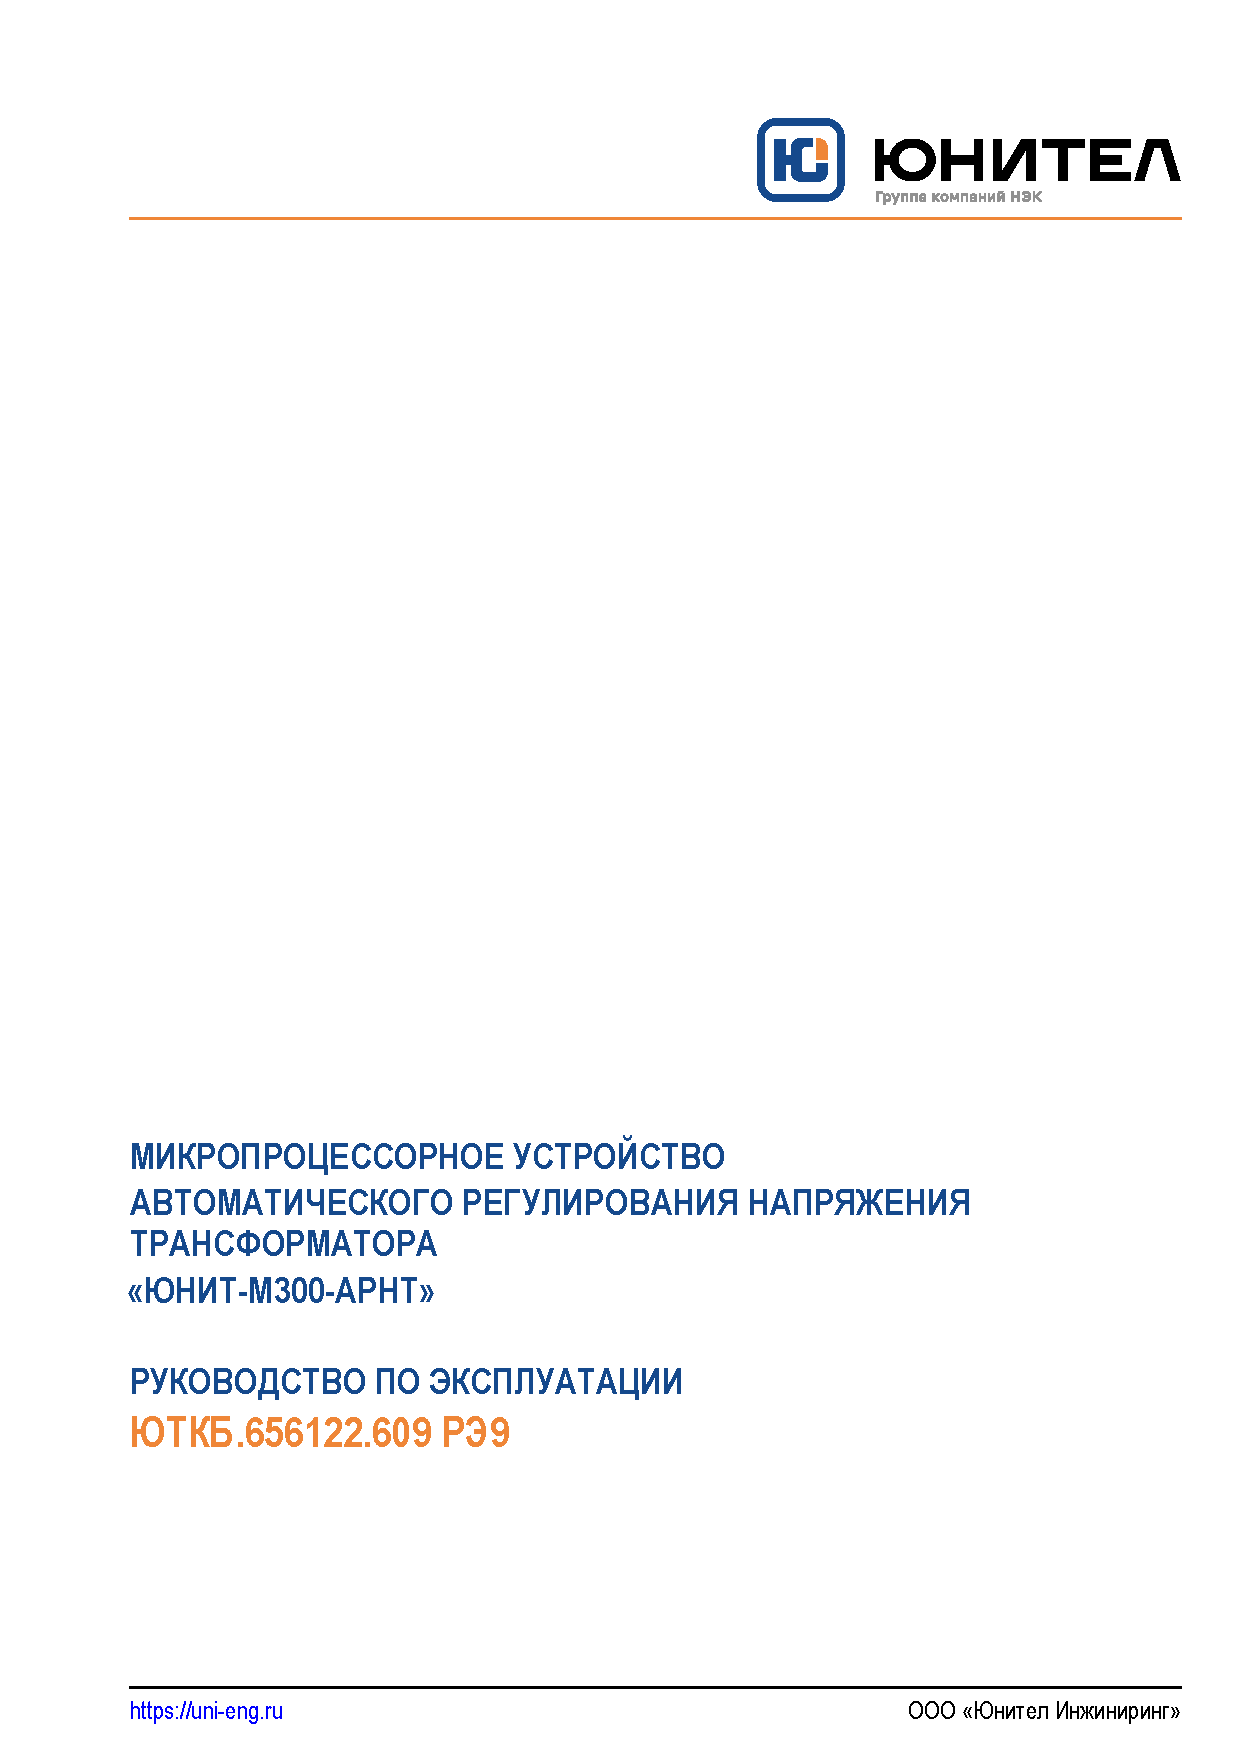
\includepdf[pages={1},width=0.5\textwidth, angle=90]{1.pdf} вставляем и поворачиваем pdf
%\begin{center}
%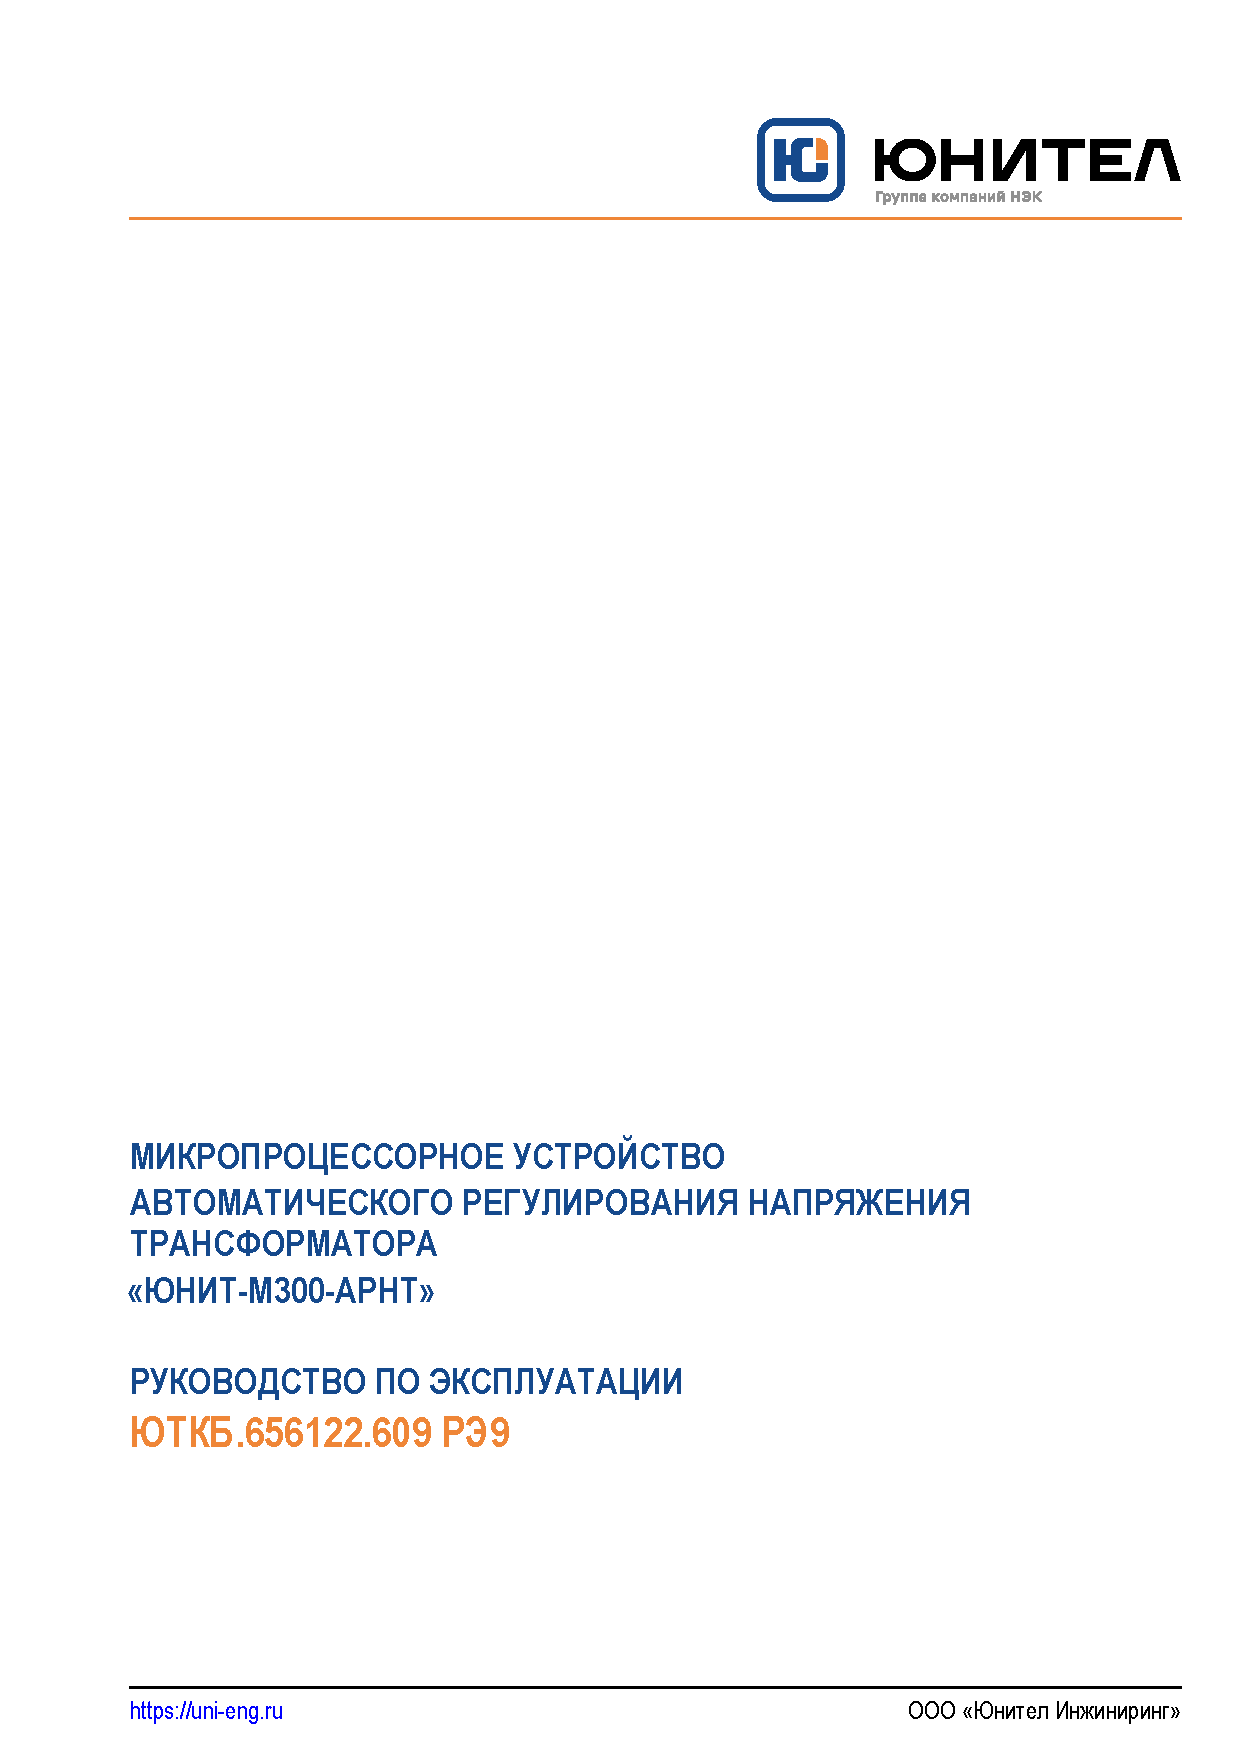
\includegraphics[width=1.4\textwidth]{1.pdf}
%\end{center}

\end{landscape}
\restoregeometry

